\newcommand{\modelname}{LTAG}
\chapter{基于Transformer编码器-解码器结构的自动歌曲翻译}
\label{sec:ast}
本章将详细介绍本文在自动歌曲翻译研究中使用的数据、提出的模型和实验结果。本章首先说明了使用的单语言数据集来源、收集双语平行数据集的方法,并提出一种基于神经机器翻译中常用的Transformer的编码器-解码器结构的歌词和歌词-旋律对齐共同翻译框架,并在此基础上设计了一系列实验来检验模型框架的表现。实验结果显示,本章提出的框架相比其他自动歌曲翻译算法,在歌词文本翻译质量和歌曲翻译整体演唱效果上都取得了更好的效果。
\section{自动歌曲翻译模型结构}
\begin{figure}[ht]
    \centering
    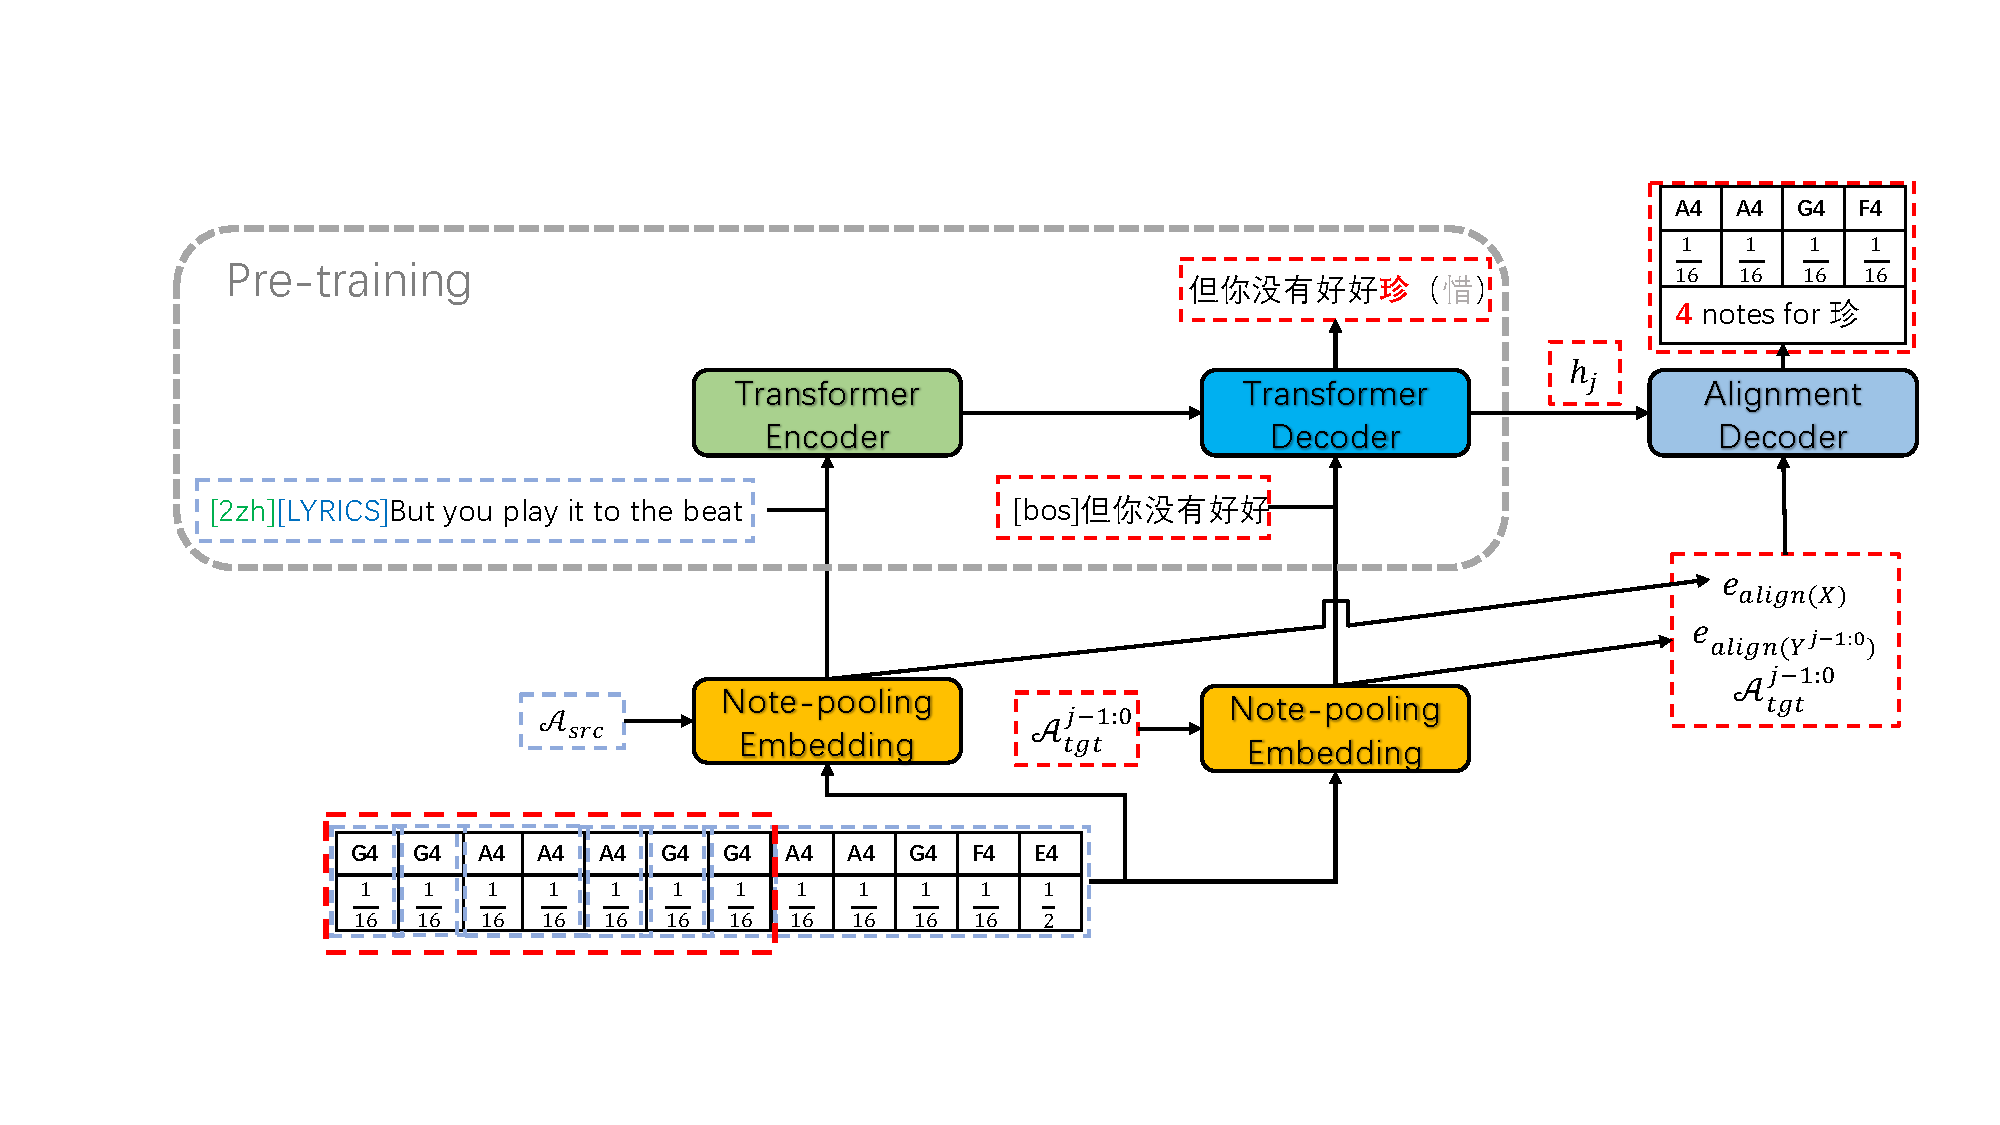
\includegraphics[width=0.99\textwidth]{figure/ast/pipeline.pdf}
    \caption{本章提出的模型架构概览,图示以第$j$个解码时间步进行了说明。Transformer解码器将输出目标语言的词语,对齐解码器会输出对齐音符的数量。}
    \label{fig:model}
\end{figure}
本章设计的模型属于神经机器翻译中常用的自回归翻译架构,但与一般的翻译模型不同的是,它能同时进行自回归的歌词文本翻译和歌词文本与旋律的对齐预测。
如图\ref{fig:model}所示,它由用于歌词翻译的基于Transformer Encoder-Decoder的子结构、两个音符表示池化嵌入层和一个对齐解码器组成。
基于Transformer的编码器-解码器部分参考了\citet{gagast}中的做法,使用去噪自编码器~\citep{bart}和翻译作为预训练任务。
在预训练期间,由于混合使用了单语言和双语翻译数据,且数据文本来自新闻、书本和歌词等多个领域,两个分别表示翻译方向和文本域的前缀词语会被添加到源语言的输入句子里以建立模型区分翻译方向和目标文本所属文本域的能力。
模型整体由用于结合歌词-旋律对齐编码旋律信息的音符表示池化嵌入层、Transformer的编码器-解码器的歌词翻译模块和歌词-旋律对齐的解码器部分组成。
音符表示池化嵌入层的结构如图~\ref{fig:align_enc}所示,这是一个用于处理歌曲旋律信息的模块。
图~\ref{fig:align_dec}中的对齐解码器则是基于本章后提出的节的自适应音符分组方法构建,该方法在自回归解码期间能动态预测与当前解码时间步预测出的的词语相对齐的音符数量。下面将详细介绍这些模型的组成部分。
\subsection{基于Transformer的编码器-解码器结构}
\label{sec:transformer_enc_dec}
\subsection{音符表示池化嵌入层}
\label{sec:note_pooling}
音符表示池化嵌入层将音符和音符与歌词词语的对齐信息作为输入,并输出池化后的音符嵌入表示和对齐嵌入表示。
输入的旋律音符序列由MIDI格式的音高和每个音符的持续时间两部分组成。每一个音符的持续时间都是离散的谱面时长的一类:四分音符、半音符或八分音符等。
\begin{figure}[t]
    \centering
    \label{fig:align_enc}
    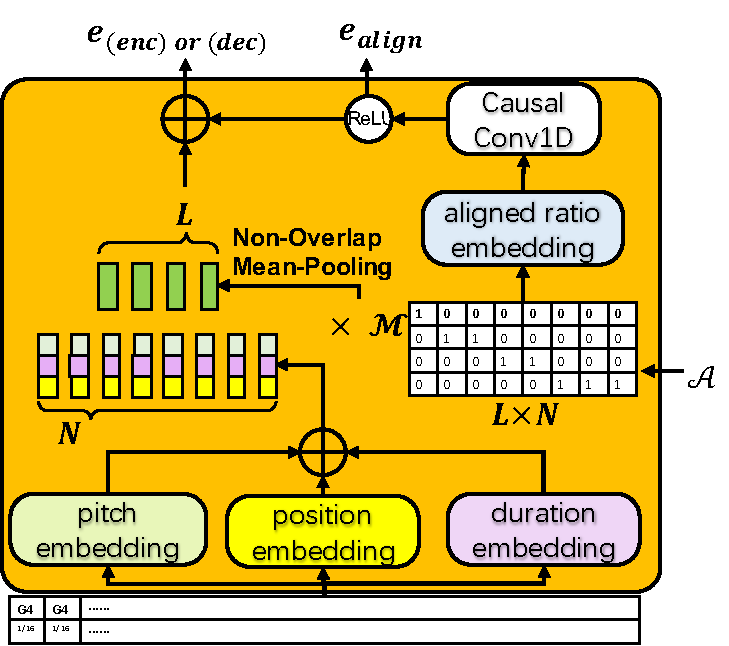
\includegraphics[width=0.69\textwidth,clip=true]{figure/ast/note-pooling.pdf}
    \caption{音符表示池化嵌入层结构图示。该层会根据音符序列的表示和对齐信息进行编码。}
\end{figure}
音符的MIDI音高和持续时间可以分别表示为嵌入表示$e_{midi}$和$e_{dur}$。
定义第$i$个音符的嵌入表示为:
\begin{equation}
\label{eq:note}
    \mathbf{e}_{note}^i=\mathbf{e}_{midi}^i+\mathbf{e}_{dur}^i+\mathbf{e}_p^i
\end{equation}
其中,$\mathbf{e}_p^i$是位置嵌入表示,来自于序列顺序位置$i$。
池化嵌入层会根据对齐信息,对音符的嵌入表示序列进行互不重叠的平均池化操作。具体而言,就是将对齐到同一词语的连续的一段音符序列的嵌入表示进行平均。下面给出公式化的表达,对齐信息$\mathcal{A}$会被表示为一个01矩阵$\mathbf{M} \in \{0,1\}^{L \times N}$,其中$L$和$N$分别表示文本序列和音符序列的序列长度。如果第$i$个音符对齐到了第$j$个词语,那么$\mathbf{M}_{ji}=1$,否则$\mathbf{M}_{ji}=0$。
这样,$\mathbf{M}$就能直接通过张量间的矩阵乘法快速有效地进行互不重叠的平均池化操作,其结果记为旋律嵌入表示$\mathbf{e}_{md}$。
\begin{equation}
\label{eq:md_embed}
    \mathbf{e}_{md} = \text{Non-Overlap-Mean-Pool}(\mathbf{e}_{note}, \mathbf{M})
\end{equation}
有音符嵌入表示$\mathbf{e}_{note} \in \mathbb{R}^{N \times d}$($d$ 是嵌入表示张量的维度)和对齐矩阵$\mathbf{M} \in \{0, 1\}^{L \times N}$.
那么互不重叠的平均池化操作可以按照如下计算进行:
\begin{align*}
\mathbf{W} &= \mathbf{M} / \text{sum}(\mathbf{M}, \text{dim}=-1, \text{keepdim}=\text{True}) \\
\mathbf{e}_{md} &= \mathbf{W} * \mathbf{e}_{note}
\end{align*}
其中,$/$代表矩阵按元素相除,$*$代表矩阵相乘。
通过pytorch支持的\texttt{gather}和\texttt{scatter}张量操作,上述互不重叠的平均池化操作就可以在训练时的小批次数据中进行了。
由上述说明易知,此池化操作的核的尺寸大小不是固定的,而是随着01矩阵$\mathbf{M}$的行的和变化而变化。

进一步说,由于歌词-旋律的对齐是单调的,即歌谱中每个音符只能对应一个词语,通过计算对齐音符的数量的累积和就可以更简洁地编码对齐情况:
\begin{equation}
\label{eq:cumsum}
    \mathbf{s} = \text{CumSum}(\text{RowSum}(\mathbf{M}))
\end{equation}
其中,$\mathbf{s}$是一个长度为$L$的整数向量。那么$s^j / N$就表示每个对齐音符的\textbf{对齐比率}。
接下来,通过将累积对齐比率分组为$(0,1]$范围内的大小相等的区间就可以将比率离散化,并引入一组嵌入表示张量$\mathbf{E}_{ratio}$来表示每个区间。划分成的区间数是一个可调节的超参数。所以,对齐比率嵌入表示的计算方法如下:
\begin{align}
\label{eq:align}
    \mathbf{e}_{align}^j = f(\mathbf{E}_{ratio}(s^j / N))
\end{align}
其中,$f(\cdot)$是一个简单的非线性神经网络层,由一维因果卷积层和ReLU激活函数组成。
最后,将旋律嵌入表示和对齐比率嵌入求和,结果被输入到基于Transformer的子结构的编码器或解码器,和其中原有的嵌入表示相加:
\begin{equation}
\label{eq:embed}
    \mathbf{e}_{\text{enc(dec)}} = \mathbf{e}_{token} + \mathbf{e}_p + (\mathbf{e}_{md} + \mathbf{e}_{align})
\end{equation}
如公式~(\ref{eq:md_embed})所示,每个旋律嵌入表示都会对应于该段旋律对齐到的词语。
此外,使用因果卷积层意味着音符对齐比率的嵌入张量也具有与文本序列相同的长度,并且能够保证每个对齐比率的嵌入表示仅以自回归的方式与先前的比率嵌入表示相关。上述性质就保证了该层在解码器中可以完美地适应自回归方式的翻译需要进行的Teacher-forcing式训练。
来自源端歌词的对齐嵌入表示由于在解码时并没有目标端的词语可以对去,所以这部分会整体经过池化层处理以形成全局的对齐参考表示,并输入到对齐解码器中。
本章提出的这种设计的动机在于用对齐的音符数来隐式地对歌词的翻译过程进行限制。

\subsection{对齐解码器的结构}
受自适应计算时间方法(Adaptive Computation Time,ACT)~\citep{act}的启发,本章提出了\textbf{自适应分组}模块来对歌词和音符的对齐情况进行建模。
如图\ref{fig:align_dec},\ref{fig:act_gp}所示,此模块能够预测出应将多少个连续的音符分配给当前解码时间步正在处理的词语。
\begin{figure}
\subfloat[The alignment decoder]{
    \label{fig:align_dec}
    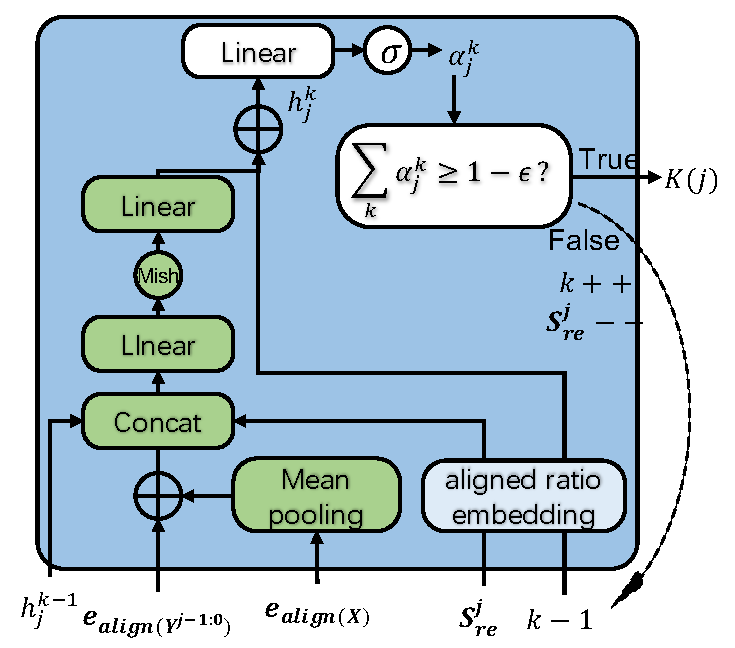
\includegraphics[width=0.49\textwidth,clip=true]{figure/ast/alignment_decoder.pdf}
}
\subfloat[Adaptive grouping process]{
    \label{fig:act_gp}
    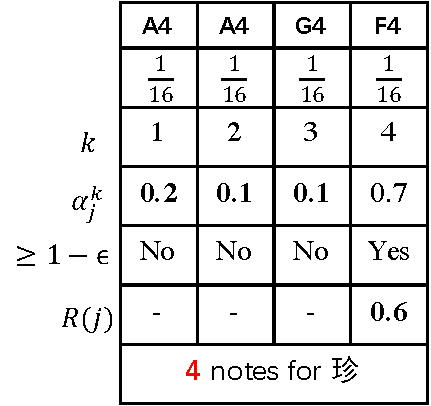
\includegraphics[width=0.49\textwidth,clip=true]{figure/ast/act_gp.pdf}
}
  \caption{对齐解码器的结构图示和工作过程。对齐解码器能根据停止概率的分布计算对齐音符的数量。}
\end{figure}
自适应计算时间方法
\subsubsection{自适应音符分组预测}
\label{subsec:act}
一般地,有$1 \leq j \leq L_Y$,设$y_j$为第$j$个目标端文本词语,$\mathbf{h}_j$为基于Transformer的解码器的最后一层相对应的隐层表示。
为了说明之便而又不失一般性,假设之前的文本序列$y_{j-1:0}$已经与前$n-1$个音符完成对齐,下文将通过遍历一个索引变量$k$($k$从1开始)来定义自适应音符分组预测与$y_j$对齐的音符数量的过程。
\begin{align}
    \mathcal{S}_{re}^j &= N -s^{j-1}_{tgt} \\
     \mathbf{h}_j^0 &= \mathbf{h}_j  \\
     \mathbf{h}_j^k &= g(\mathbf{h}_j^{k-1}, \mathbf{e}_{align(X)}, \mathbf{h}_{align(y_{j-1:0})}, \mathcal{S}_{re}^j, k-1) \\
     \alpha_j^k &= \sigma(\text{Linear}(\mathbf{h}_j^k))
\end{align}
其中,$\mathbf{e}_{align(X)}$是完整的来自源语言端的对齐嵌入表示,$\mathbf{e}_{align(y_{j-1:0})}$则是已经过解码的先前部分的对齐嵌入表示,$s^{j-1}_{tgt}$是$\mathbf{s}$向量中的第$j$元素($\mathbf{s}$来自公式~(\ref{eq:cumsum})。
现在模型既有每句歌词对应的完整旋律中的音符数量信息,又有已经对齐到目标端的音符数量,那么可以计算当前解码步骤中第$j$时间步时,剩余未对齐音符的数量为$\mathcal{S}_{re}^j$。如上文所述,$\mathbf{e}_{align(X)}$经过一个平均池化层以获得单个向量表示作为全局参考,从而使得来自源语言端的对齐情况始终可以与可变长度的目标端的$\mathbf{e}_{align(y_{j-1:0})}$进行加和。
一个多层神经网络$g(\cdot)$会对所有的输入进行处理,具体网络结构如图\ref{fig:align_dec}中绿色部分所示。
最后,经Sigmoid函数$\sigma(\cdot)$处理,模块会这一步处理中间态的自适应分组停止概率$\alpha_j^k$。
所有中间态停止概率的总和表示当前$k$个音符与目标端词语$y_j$对齐的可能性。

给定一个超参数$\epsilon$,通常为一个很小的浮点数(例如,0.01),如果此时的$k$满足$\sum_k \alpha_j^k < 1-\epsilon$,即累计概率未超过阈值,那么自适应分组过程会继续进行并将$k$递增为$k=k+1$;相应递减$\mathcal{S}_{re}^j=\mathcal{S}_{re}^j-1$,然后进行上述计算。
否则,累计概率已经超过了既定阈值,对齐预测的分组过程停止,对齐解码器输出当前对齐的音符数$K(j)$。
\begin{equation}
\label{eq:Kj}
    K(j) = \underset{K}{\mathrm{argmin}} \left\{\sum_{k=1}^K \alpha_j^k \geq 1-\epsilon \right\}
\end{equation}
在$\epsilon$是正值$\epsilon>0$的情况下,这个预测过程能确保$K(j)\geq1$,也就是说对于每个词语,至少有一个音符会被对齐到该词语上。
为了清晰地定义对齐$K(j)$个音符到当前词语的概率,引入一个余项$R(j) = 1-\sum_{k=1}^{K(j)-1} \alpha_j^k$。
这样,$\alpha_j^k$和$R(j)$就都可以是有效的概率分布了。
图\ref{fig:act_gp}是本节提出的自适应分组方法在歌词音符对齐预测上运行的一个示例。
\begin{equation}
\begin{array}{rl}
    L_G = & \left| \sum_j K(j) - N \right| + \sum_j \left|K(j) - \Delta_j\right| \\
    \approx &\left|\sum_j \left(K(j) - (1 - R(j))\right) - N \right| \\
    & + \sum_j \left|K(j) - (1 - R(j)) - \Delta_j\right|
\end{array}
\end{equation}

\subsubsection{自适应分组模块的梯度计算}
本小节将详细阐述\ref{subsec:act}小节中介绍的自适应分组算法的优化过程,由于算法运行过程是求满足$\sum_{k=1}^K \alpha_j^k \geq 1-\epsilon$的$k$的最小值,该过程本身不可导,所以对算法中使用的神经网络参数的优化和梯度计算需要一些技巧。
在人工标注的歌词-旋律对齐数据中,每个目标端文本序列的词语所对齐的音符数的真实值都被标注出来了,这里先将序列中第$j$个词语对齐的此值记为$\Delta_j$。
与自适应计算时间方法\citep{act}原文中最小化``思考成本''$\sum_j K(j) + R(j)$不同的是,本节提出的自适应分组算法会通过最小化下面这项自适应分组损失$L_G$来优化参数。这种做法会通过引入$\Delta_j$来自然地限制目标端文本序列中每个词语的``思考成本''的上界。
\begin{equation}
\begin{array}{rl}
    L_G = & \left| \sum_j K(j) - N \right| + \sum_j \left|K(j) - \Delta_j\right| \\
    \approx &\left|\sum_j \left(K(j) - (1 - R(j))\right) - N \right| \\
    & + \sum_j \left|K(j) - (1 - R(j)) - \Delta_j\right|
\end{array}
\end{equation}
显然,变量$K(j)$的计算方式对于停止概率是不连续的,因此模型在优化时近似使用了$1-R(j)$项以使自适应分组损失可微。
根据上述自适应分组损失的定义,其实只需要分析以下项对预测对齐音符数的作用:
\begin{equation}
    \left| K(j) - (1 - R(j)) - \Delta_j \right|
\end{equation}
1)如果在正向传播过程中,$K(j) > \Delta_j$,则由于本节提出方法的设定,$K(j)$和$\Delta_j$都是正数,所以有$K(j) - \Delta_j \geq 1$。
那么,为了最小化自适应分组损失,$1 - R(j)=\sum_{k=1}^{K(j)-1}\alpha_j^k$就应该被调整得更大。
也就是说,此时,优化过程会将$\sum_{k=1}^{K(j)-1}\alpha_j^k$这一项逐渐推向$K(j) - \Delta_j$。
Note that the theoretical upper bound of $\sum_{k=1}^{K(j)-1}\alpha_j^k$ is $K(j)- 1$, which is larger or equal to $K(j)- \Delta_j$.
因此,这种情况下对参数的优化是有效的,并且在优化期间将满足以下条件:
\begin{equation}
    \sum_{k=1}^{K(j)-1}\alpha_j^k \geq 1 - \epsilon
\end{equation}
根据前文中对$K(j)$的定义,可以得出以下结论:
\begin{equation}
    K(j)^{\text{new}} = \arg\min_{K}\left\{\sum_{k=1}^K \alpha_j^k \geq 1 - \epsilon\right\} \leq K(j) - 1
\end{equation}
2)如果有$K(j) < \Delta_j$,相应过程的推导分析也是类似的。这种情况下,要将$\sum_{k=1}^{K(j)-1}\alpha_j^k\rightarrow0$往减小自适应损失的方向推,也就意味着如果第$K(j)$个计算得出的停止概率仍不满足$\alpha_j^{K(j)} \geq 1-\epsilon$的条件,那么$K(j)^{\text{new}}$就会在优化过程中呈增大趋势。
然而,如果有$\alpha_j^{K(j)} \geq 1 - \epsilon$,优化就会停止。
所以可以优化$\left| K(j) - \left(1 - R(j) + \alpha_j^{K(j)}\right) - \Delta_j \right|$,即,$\left| K(j) -\sum_{k=1}^{K(j)} \alpha_j^{k} - \Delta_j \right|$。
虽然有以上分析结果,但是在实际训练中的观察发现,这种情况其实非常罕见,几乎不会出现。就算出现,在训练仅进行几个周期后,这种现象就会完全消失。
因此,在训练中可以仍然采用了上述1)情况中同样形式的自适应分组损失。
3)如果有$K(j) = \Delta_j$,那么此词语对应的损失项在自适应分组损失中就可以完全不起作用,无需其他讨论。

此外,由于与多个音符对齐的词语在歌曲中属于少数,因此在实际训练时,来自于这些词语的对齐损失会被加上更大的权重来让优化更多地关注这些重点部分的对齐预测情况。
\section{基于Back Translation的数据增强}
\label{sec:bta}
虽然本章中收集的规模在上千句左右的歌曲数据集能够初步满足训练模型的需求,其中包含的来自人工翻译平行双语歌词和歌词-旋律对齐信息的标注数量是非常有限的,而且这对标注人员素质提也提出了较高要求,因此对于实际应用会有收集耗时较长,代价昂贵的问题。

所以,本章还改造了近年来神经机器翻译研究中广泛使用的基于回译的数据增强方法\citep{backtrans}来生成更多的双语歌曲训练数据。
相比于本章提出的人工标注的平行双语歌曲数据集,在公开网络上显然可以搜集到数量更为庞大的单语歌曲数据。通过构建一个可以进行长度控制的预训练歌词翻译模型,目标语言中的单语数据就能被回译到源语言中。
长度控制可以确保翻译出的结果的词语的数量与所对应的旋律的音符数量相同,这样就能在源语言端制造歌词和音符的简单一对一对齐。
经过如此改造后的回译方法就能够制造出相对较大的双语歌曲数据集。显然,这样增强出的数据在源端有信息噪声,但在目标端仍然保留了非常准确的信息。
由于回译出的数据比人工标注的数规模大得多,本章在实际训练中采用了类似课程学习的方式来进行训练时的数据采样。即在训练初期,来自回译增强的数据将与来自人工标注的数据真实数据混合。人工标注的数据被上采样到与回译数据差不多的数量级,
对回译数据的降采样率则会随训练进行不断减小,这样,每个小批次训练数据中人工标注数据的占比就会随着训练的进行不断提高。具体来说,回译产生的数据的下采样率从1.00开始,在总训练周期的一半时下降到0.01。
人工标注的数据的采样率从20.00开始进行上采样,并在总训练周期结束时降至5.00。

\begin{figure}[htbp]
    \centering
    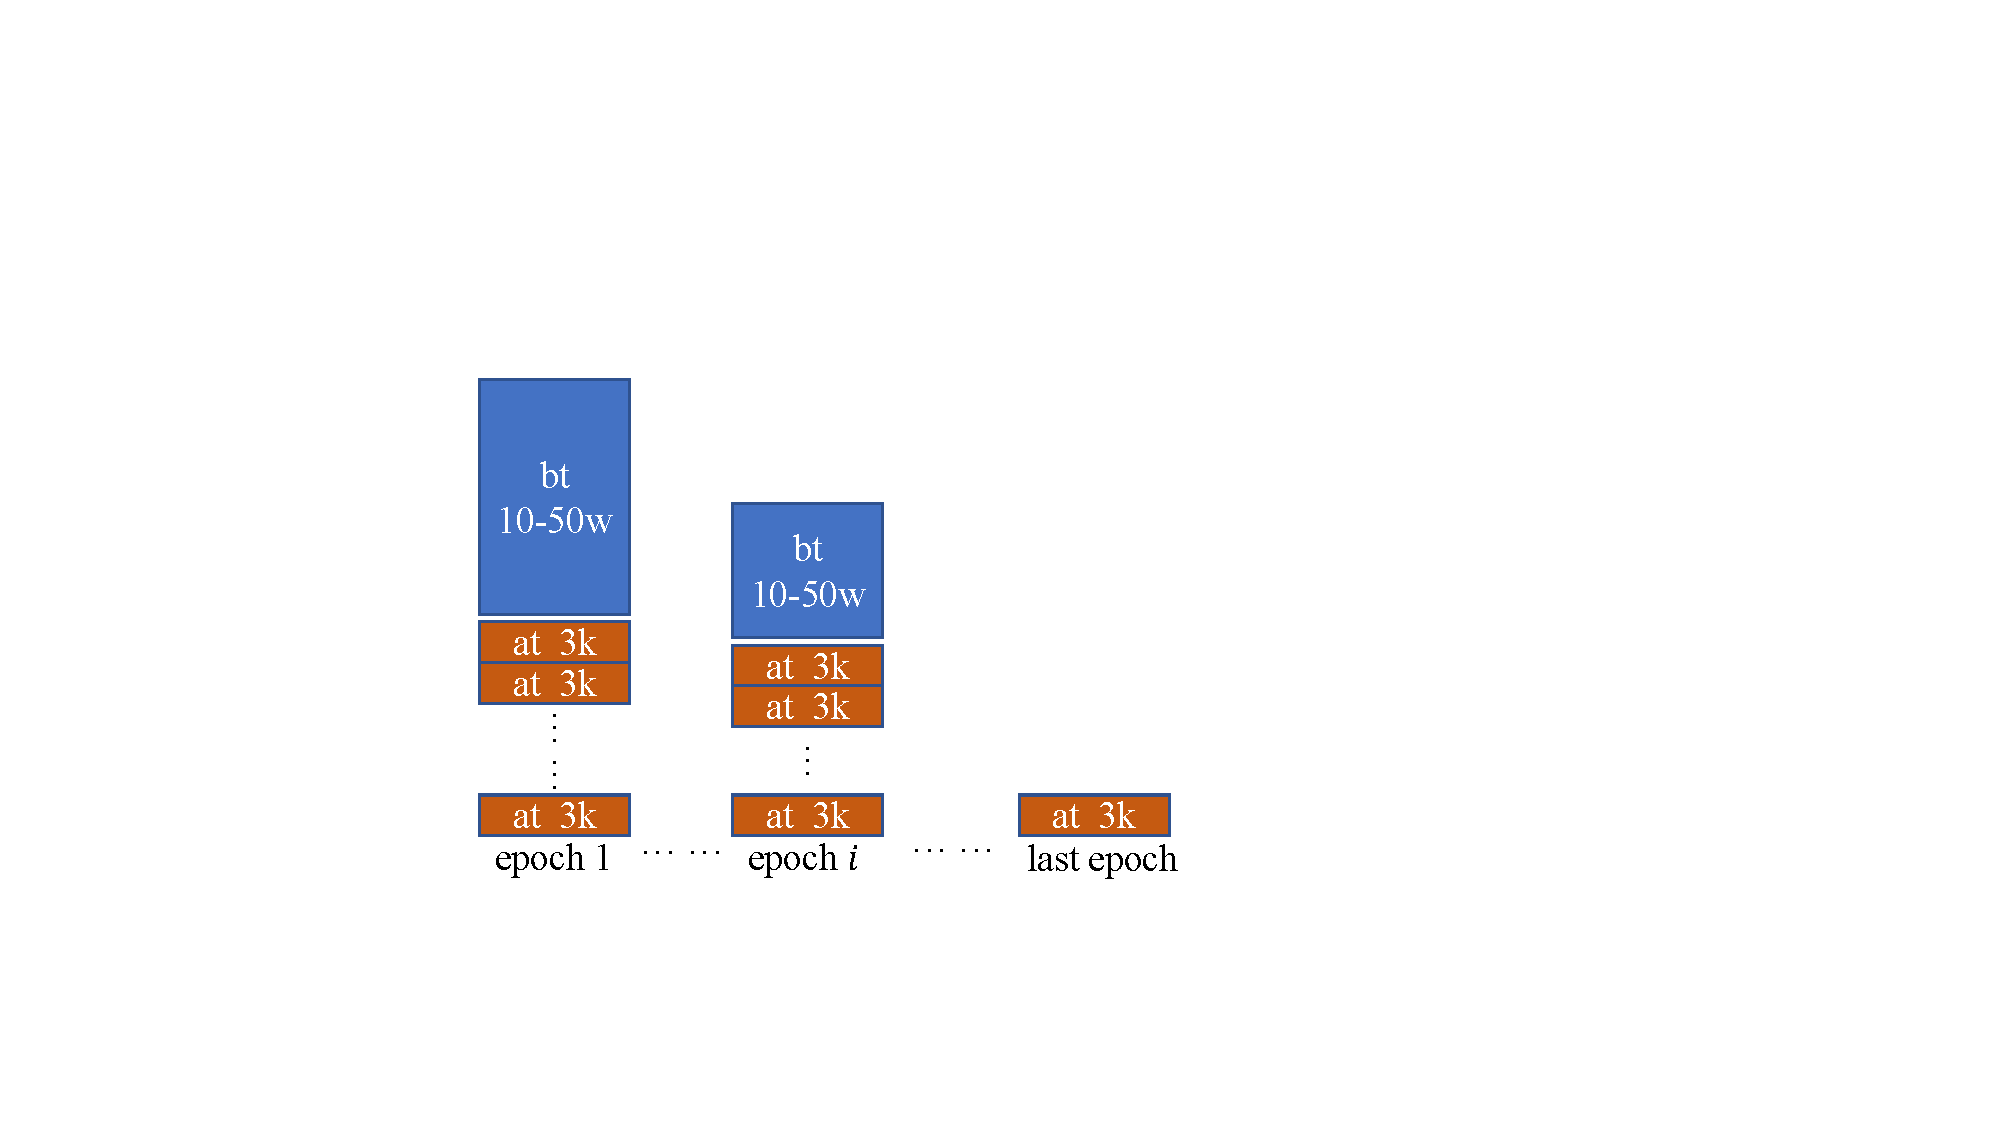
\includegraphics[width=0.5\textwidth]{figure/ast/backtrans_curriculum.pdf}
    \caption{如何在歌词和歌曲-旋律对齐的共同翻译训练中使用回译数据和带注释的数据的图示说明。``bt''表示来自back-translation回译数据增强得到的数据,``at''表示来自人工标注的准确歌曲数据。}
    \label{fig:bt_curriculum}
\end{figure}
\section{歌曲翻译的评价指标}
\label{sec:metric}
对本章提出的模型所针对的自动歌曲翻译任务的表现的评价,最有说服力的指标就是翻译后的歌曲结果是否能被正常演唱、歌词文本易于理解,以及,最核心的指标,是否仍和原歌曲一样是人类乐于欣赏的歌曲作品。
因此,本章的实验评测参考了\citet{songmass}~中的做法:在进行人工评测时,评测人员会根据展示出的模型翻译结果——歌词和歌词-旋律对齐情况制成的歌谱,给出评测打分。
但是由于本章所针对的自动歌曲翻译任务的特殊性,为了以一种接近实际中端到端的方式验证翻译结果的可唱性,本章的实验评测还使用了一个开源的歌唱语音合成模型~\citep{diffsinger}为评测人员提供翻译后歌曲的演唱音频,期望以此让标注人员进行更直观的演唱评测。

进行人工测试的歌谱和声音是由测试集中随机得到的20个片段,并展示乐谱和合成歌声
对于翻译质量的自动评测,本章采用了sacreBLEU\footnote{\url{https://github.com/mjpost/sacrebleu}}分数。
对于歌曲翻译的可理解度、翻译后歌曲的自然度、可唱性和整体质量评估,本章采用了人工评估,使用平均意见得分~(Mean Opinion Score,MOS),三项分别对应分数MOS-T、MOS-S和MOS-Q。
在自动评估对齐情况时,机器翻译领域中常用的对齐错误率(Alignment Error Rate,AER)却并不适用于此,因为除了模型生成的需要评测的歌曲-旋律对齐之外,目标端的歌词翻译结果也是机器生成的。
于是,本节提出了一种对齐分数(Alignment Score,AS),用于计算预测的歌词-旋律对齐和真实情况之间的在测试集上的统计频率的加权交(Intersection over Groundtruth,IOG):
\begin{equation}
    % \text{AS} = \frac{\sum_{k} \min(\text{freq}_{pred}^k, \text{freq}_{gt}^k) * k)}{\sum_{k} \text{freq}_{gt}^k * k }
    \text{AS} = \frac{\sum_{k}\min(\text{freq}_{pred}^k/F_{pred}, \text{freq}_{gt}^k/F_{gt}) * k)}{\sum_{k} (\text{freq}_{gt}^k/F_{gt}) * k) }
\end{equation}
式中$k$即为前文中的对齐音符数,而$F = \sum_{k} \text{freq}^k$是频率的总和。对齐分数反映的是预测的歌词-旋律对齐的分布和真实歌曲的歌词-旋律对齐的分布的相似程度,是在同一有一定规模的测试集上的整体评价指标,不常见的歌词-旋律一对多情况对相似度的贡献会随音符数增大。
\section{实验设计}
\subsection{歌曲翻译数据集}
目前,在歌曲翻译研究领域并没有高质量的平行歌词翻译和歌词-旋律对齐的公共数据集可用,所以本文收集并标注了一个数据集PopCV(Pop songs with Cover Version),该数据集包含若干中文歌曲的英文翻唱版本和英文歌曲翻唱版本。除此以外,本文还使用了一些单语言歌曲语料, 包括一个英文歌词和歌词-旋律对齐数据集LMD\footnote{\url{https://github.com/yy1lab/Lyrics-Conditioned-Neural-Melody-Generation}}~\citep{LMD},以及一个从唱吧App上爬取的一些中文歌曲语料。
两组单语言歌曲数据仅被用于训练模型,测试数据是在经专业标注人员标注的真实数据上进行的。数据集概述见表\ref{tab:dataset_stat}.
\begin{table}[htbp]
    \centering
    % \setlength{\tabcolsep}{2pt}
    \begin{tabular}{|l|c|c|c|c|}
    \hline
         & 语种 & 歌曲数(首) & 歌词数(句) & 数据来源和实验用途\\
    \hline
     LMD & 英文 & \diagbox[]{}{} & 152,991 & 回译\\
    \hline
     唱吧 & 中文 & \diagbox[]{}{} & 542,034 & 回译\\
    \hline
     PopCV & 中文、英文 & 79 & 2,959 & 标注\\
    \hline
     测试集 & 中文、英文 & 25 & 629 & 标注\\
    \hline
    \end{tabular}
    \caption{本文中所涉及的歌曲翻译数据集的数据统计情况。}
    \label{tab:dataset_stat}
\end{table}
\subsection{歌曲翻译数据收集流程}
由于此类歌曲翻译的数据集并没有行业标准或其他公开发布的先例,于是,本文首先设计了一个相对省时,且对于标注员来说,比较容易执行的标注过程。
首先,从一些公开的乐谱网站收集歌曲的乐谱文件\footnote{\url{https://www.musescore.com} 和 \url{https://wwww.midishow.com}}.
然后,专业标注人员会根据歌曲在原版和翻唱版本中的演唱方式,按照一般的歌谱编纂规则的指示\footnote{\url{https://lilypond.org}和\url{https://musescore.org/howto}}将歌词添加到乐谱的音符上。歌词中的每个单字或音节会被添加在开始演唱的音符上,如果有延音情况,
后续的音符上会标注下划线``\_\_''字样,如果有同词的不同音节分在了不同音符进行演唱,
会使用短划线``-''进行连接。
例如了两个相邻不同音符的``fam$-$''、``$-$ily''就表示``family''一词以两个音节进行了演唱。
然后,标注好的乐谱文件会被以\texttt{.musicxml}的格式导出,然后自动提取出歌词及其对齐的音符并整理成数据集。
\begin{figure}[t]
    \centering
    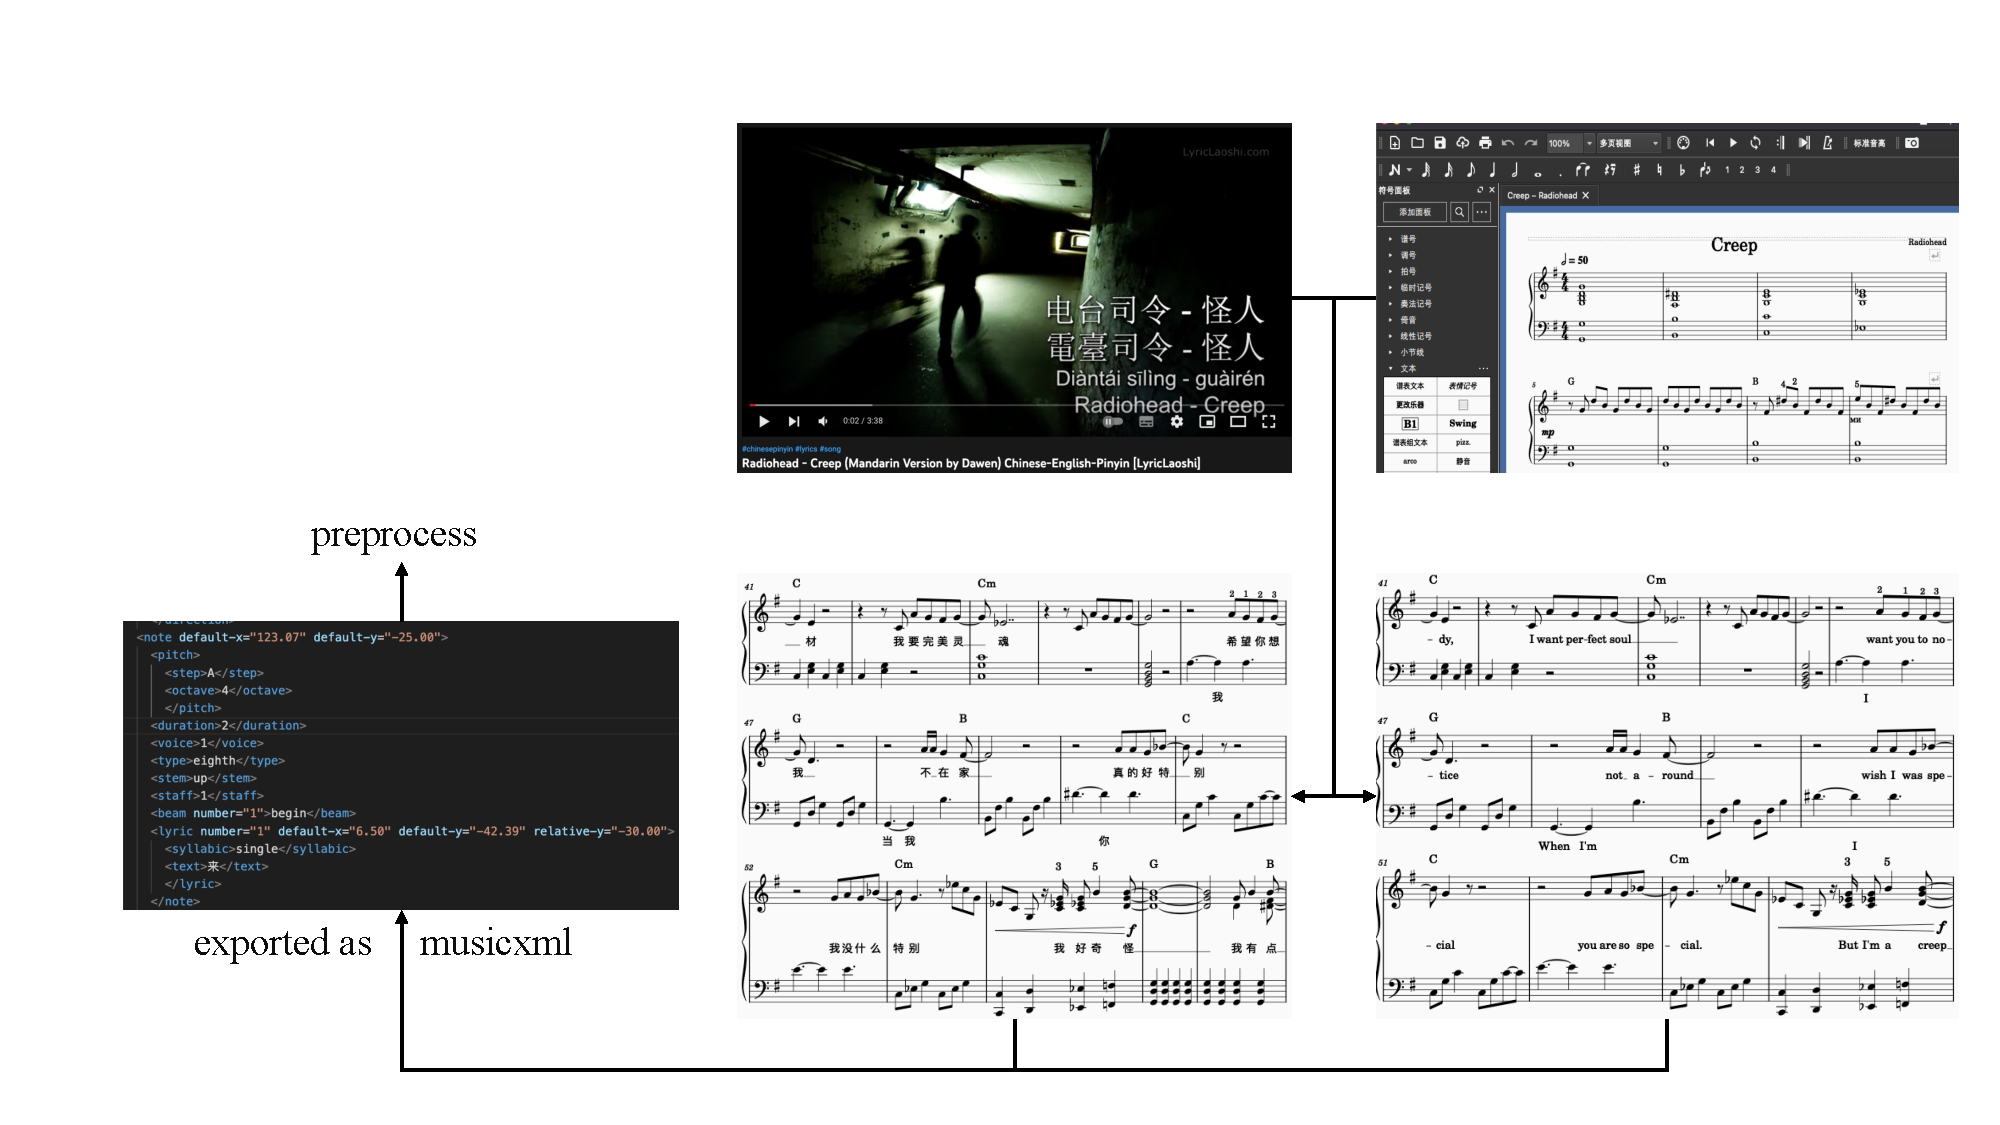
\includegraphics[width=0.99\textwidth]{figure/ast/da_pipeline}
    \caption{本文提出的歌曲翻译数据标注流程概览。}
    \label{fig:da_pipeline}
\end{figure}
乐谱的制作和到处使用的软件为musescore。
\subsection{musicxml文件解析处理}
musicxml是一种和MIDI相比相对开放自由,易于分发的记谱文件格式。musicxml文件是基于标准xml技术的,是一种文本文件而非二进制文件。musicxml显示格式有着精确的定义,因此可以做到对于同一个文件在不同的环境下打开都有着同样的谱面显示内容。musicxml中的音乐语义主要由xml式的elements表达,也就是其中的xml标签,并以标签的嵌套关系表达音乐语义的元素包含关系。本章进行数据集收集处理的musicxml文件的头部由谱子信息,xml文件信息和各声部信息组成。其中,musicxml里包含的声部信息通常包含这个声部的乐器的ID、名字,MIDI乐器编号和音量等。而标注的数据主要在之后的小节中。小节由小节内容和小节信息组成。小节信息主要包括小节的属性元素,指乐谱此小节中的一些特殊元素,如谱号、调号、记号和文字等。小节内容则是音符和嵌套的音符信息。此处主要提取的是音符的音名(Step标签)、八度位置(Octave标签)、相对长度(Duration标签)和音符类型(Type标签)。
如图\ref{fig:musicxml_exp}中显示的信息就会被整理为:C4 1/8 八分音符。
\begin{figure}[ht]
    \centering
    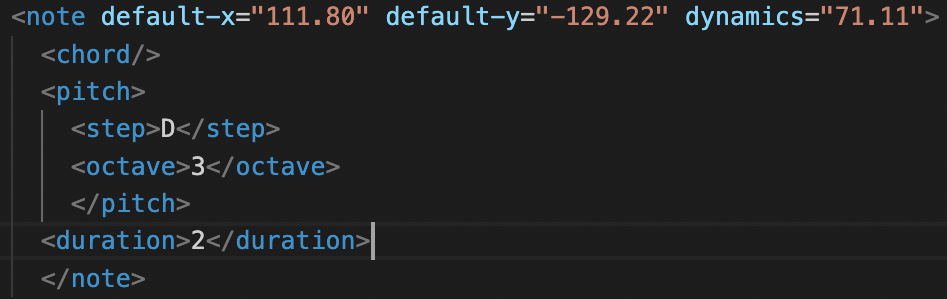
\includegraphics[width=0.99\textwidth]{figure/ast/musicxml_exp.png}
    \caption{\texttt{.musicxml}文件中涉及音符信息的标签内容示例。}
    \label{fig:musicxml_exp}
\end{figure}
音符的信息中还有一部分涉及歌词的lyric标签,其中包含了上节中说明的歌词文本标注、延音和一词多音节标注等。图\ref{fig:lyric_exp1}中的标签表示一个单字``垫''属于其所在的音符。``extend''标签表示此处歌词有延音,这时则需要向后按顺序扫描音符直到第一个没有``extend''的标签为止,此范围内的所有音符都应对齐于``垫''字。图\ref{fig:lyric_exp2}、\ref{fig:lyric_exp3}中则显示了音节之间的连接信息,``syllable''标签会的属性值只会有``single''、``begin''、``middle''和``end''。如果``syllable''标签会的属性值为``begin''
,那么则需要向后按顺序扫描音符,跳过可能出现的``middle'',直到包含``end''的歌词出现,此范围内所有音符都会按标注对齐到同一词的不同音节处。
\begin{figure}[ht]
    \centering
    \subfloat{
      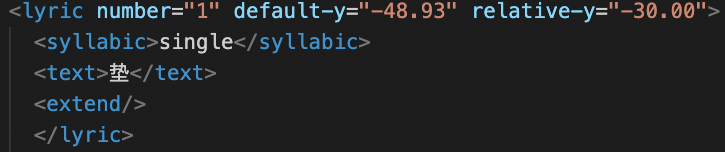
\includegraphics[width=0.99\textwidth]{figure/ast/lyric_exp1.png}
      \label{fig:lyric_exp1}
    }\\
    \subfloat{
      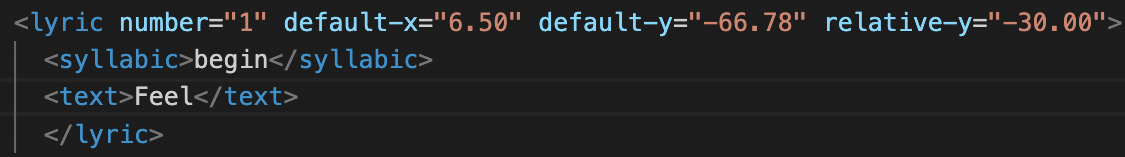
\includegraphics[width=0.99\textwidth]{figure/ast/lyric_exp2.png}
      \label{fig:lyric_exp2}
    }\\
    \subfloat{
      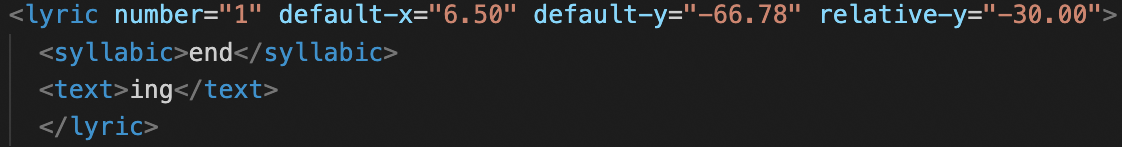
\includegraphics[width=0.99\textwidth]{figure/ast/lyric_exp3.png}
      \label{fig:lyric_exp3}
    }
    \caption{\texttt{.musicxml}文件中涉及歌词信息的标签内容示例。}
\end{figure}
总之,和musicxml相比,MIDI格式是以播放为目的,且历史悠久,所以可以搜集到的数据文件也相对较多。但是各个MIDI文件数据格式不统一,数据杂乱,对自动化处理造成了很多困难。musicxml与MIDI相比,记谱排版格式明确且是唯一的。虽然网络上原生的musicxml相对较少,由MIDI转换到musicxml意义寥寥,但是建立以musicxml为处理对象的自动化处理流程仍是必要且有意义的。
\subsection{实验设计细节}
本章进行的实验中,本章提出的模型与两个基线模型进行了对比。
其中之一是在上文中提到过的GagaST系统~\cite{gagast},该工作的主要内容是根据如中文这样的带音调语言的歌词音调限制翻译结果,并搭建了一个歌词翻译系统,在对解码过程的限制进行调整后也能适应无音调语言的歌词翻译。该工作对翻译歌词这样的特殊语体进行了适应性训练,并提出了在预训练时同时使用单语言语料和平行翻译语料以扩增可以使用的语料数量。
另一个基线模型是本章提出的模型的变体。此变体使用的是基于Transformer的编码器-解码器子结构输出的隐层表示的分类器对每个翻译出的目标端的词语的对齐音符进行预测。此模型在编码端对输入信息的编码方式和本章提出的模型完全相同,但是对齐预测使用的是比较平凡的结构。对齐预测分类的对齐音符的最大数目类别设置为30,这个量与上节阐述的对齐解码器中模型允许的出现最大$K(j)$相同。

为了生成符合音乐五线谱规则的乐谱和歌声,本章实验在对齐预测中添加了一些基于规则的后处理,以获得对模型预测结果更大的容忍度。
对于序列整体对齐音符预测总和大于旋律中音符的数量的情况,预测的对齐音符数量会被从最后一个词语到第一个词语(或从第一个词语至最后一个词语)一一减小直到预测总数和旋律的音符总数相符。
对于预测音符数量较少的情况,所有相差的对齐音符数量都会被添加到最后一个词语处。这样的规则是统一、简单又比较符合直觉的,不会对预测结果产生本质性影响。
\subsection{模型训练和实现细节}
模型整体框架中的基于Transformer的编码器和解码器会共享具有256信道维度的词嵌入表示层。
在音符池嵌入层中,MIDI音高和持续时间类型的查找表的固定大小设置为128和31。
自适应对齐解码器的分组过程的暂停超参数$\epsilon$为0.05。
对于对齐的音符大于1$\Delta_j>1$的位置,其损失函数内的权重$w_j$设置为5,而在整体的损失函数$L_{joint}$中,对齐损失的权重$\beta$设为0.8。测试时使用beam search进行搜索解码,beam的大小统一设置为5。
本章提出的\modelname~模型进行预训练时使用了基于WMT的公开翻译数据、从公开歌词翻译网站上爬取的数据和从公开歌词网站上爬取的数据进行预训练,即预训练数据包括并行语料和单语言语料。预训练时使用的语料情况如表\ref{tab:pretrain_data}所示。
\begin{table}[htbp]
    \centering
    % \setlength{\tabcolsep}{2pt}
    \caption{本文中所涉及的歌曲翻译数据集的数据统计情况。}
    \begin{tabular}{|l|c|c|c|c|}
    \hline
         & 语种 & 歌曲数(首) & 歌词数(句) & 数据来源和实验用途\\
    \hline
     LMD & 英文 & \diagbox[]{}{} & 152,991 & 回译\\
    \hline
     唱吧 & 中文 & \diagbox[]{}{} & 542,034 & 回译\\
    \hline
     PopCV & 中文、英文 & 79 & 2,959 & 标注\\
    \hline
     测试集 & 中文、英文 & 25 & 629 & 标注\\
    \hline
    \end{tabular}
    \label{tab:pretrain_data}
\end{table}
预训练时使用了4个Tesla A100 GPU进行并行训练,批最大词总数设置为20480。
对于联合翻译训练,本章使用一个Tesla V100 GPU,批最大词总数设置为4096。


对于实验评测时展示的乐谱,本节使用musescore的命令行工具对乐谱文件进行渲染并保存图片结果。图片清晰度统一为600dpi。对于模型的输出到musicxml结构,本章使用了musicly python库进行简单处理。所以展示的乐谱会缺少连音线、和弦线等一些乐谱记号,但不影响对音符和歌词标注的阅读。
\begin{figure}[ht]
  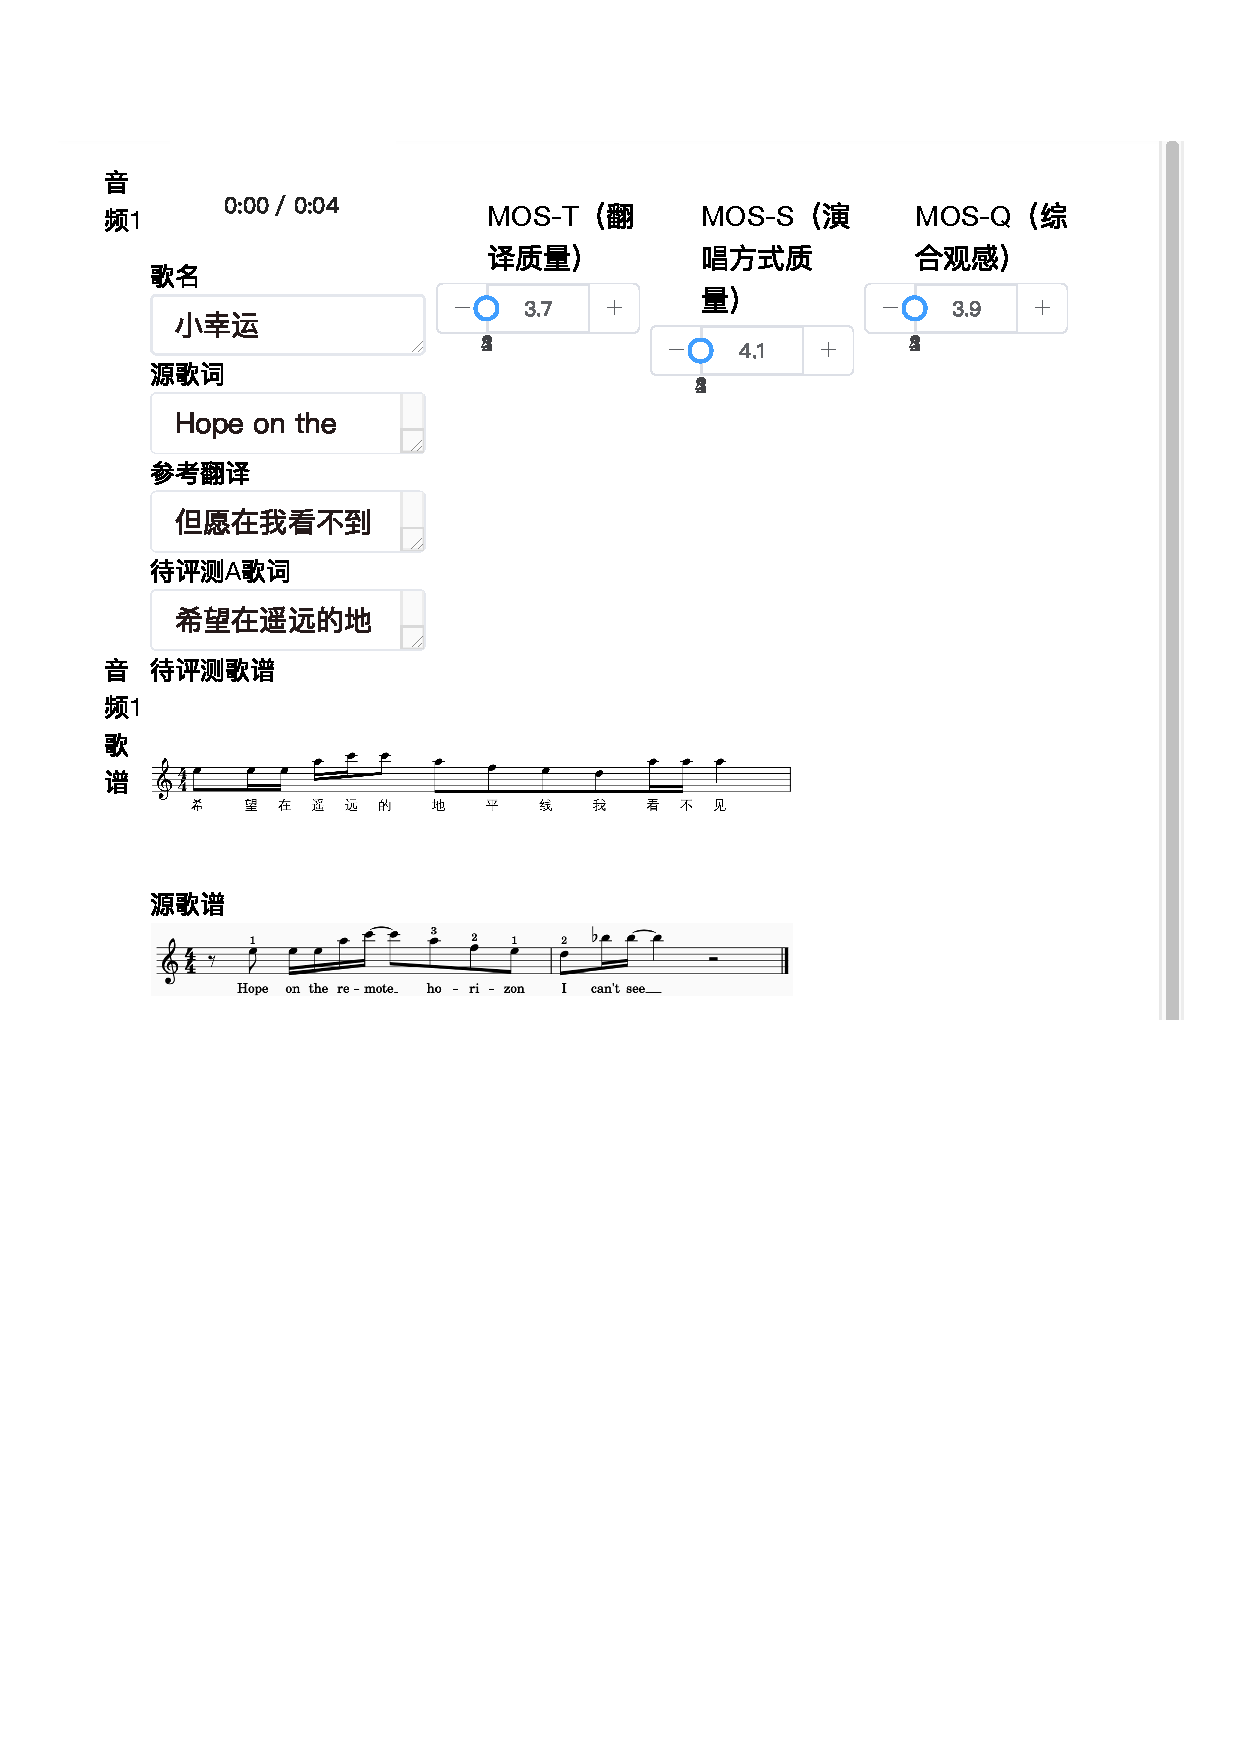
\includegraphics[width=0.99\textwidth]{figure/ast/MOS_eval_page.pdf}
  \caption{人工评测页面示例图。}
\end{figure}

对于实验评测时需要用到的歌声合成音频,本节使用\emph{pypinyin}工具(\citet{ren2020deepsinger}一文中的做法)将中文歌词的汉字转换为音素,并将hop size和frame size分别设置为128和512,采样率为24kHz。
另外,由于歌声合成模型的能力局限,所有音调在输入时都被重新调整到了C大调$A3$和$C5$之间以合成可以公平进行比较的测试用歌声音频。
为了生成符合音乐乐谱规则的乐谱和歌声,本章在模型的歌词-旋律对齐预测后添加了一些基于规则的后处理,以获得能对结果进行歌声合成的更大的容忍度,否则预测结果比和原旋律中音符数多或少这样的现象都会导致后续歌声合成模型无法以此预测结果为输入合成相应的歌声。
本章设定的后处理规则是:对于对齐预测出的音符的总数大于旋律中音符的数量的情况,将预测的对齐音符数量从最后一个词语到第一个词语或从第一个词语至最后一个词语的对齐音符数进行逐渐递减,每次减一;
对于预测音符数量和真实旋律音符数相比较少的情况,将所有相差的音符数都添加到最后一个词语的对齐上。
\section{实验结果与分析}
\subsection{主要实验结果}
本节对\modelname~和上节中阐述的其他两个基线歌曲翻译模型进行比较,并报告实验结果。
首先,表\ref{tab:subjective}中罗列了中文到英文~(Zh$\rightarrow$En)和英文到中文~(En$\rightarrow$Zh)两个翻译语向的歌曲翻译质量的人工评价指标(MOS-T)的结果。
总体上来说,本章提出的\modelname~与两个基线模型相比都得到了改进,但人工评测的实验结果也显示,模型间和不同实验设置之间的差距并不明显。
这样的实验结果部分是由于专业人士翻译歌词的结果通常是意译较多而非直译较多。那么在不同片段中,一个单词缺失可能会对人工评价的结果造成负面、中性甚至正面的影响,只有较明显的语义偏差或语法错误会导致分数在一定程度上下降。
正如在节\ref{sec:metric}中所讨论的,自动评测指标sacreBLEU应该不是比较歌词的机器翻译质量和自由翻译质量的合适的衡量标准。
\begin{table}[tbp]
    \centering
    \caption{两个翻译方向上的sacreBLEU分数和对齐分数结果。(*表示行内第二优的结果。)}
    \begin{tabular}{l|c|c|c|c}
    \hline
    \multirow{2}{*}{模型名称} & \multicolumn{2}{c|}{BLEU$\uparrow$} & \multicolumn{2}{c}{AS. $\uparrow$}\\
    \cline{2-5}
    & En$\rightarrow$Zh & Zh$\rightarrow$En & En$\rightarrow$Zh & Zh$\rightarrow$En \\
    \hline\hline
    GagaST & 11.87 & 5.67 & 0.701 & 0.468\\
    \hline
    \modelname-cls & 14.21 & 10.01 & 0.827 & 0.555\\
    ~~~ only bt  & 15.54 & 10.21 & 0.709 & 0.667\\
    ~~~ w/o bt & 13.73 & 8.26 & 0.704 & 0.490 \\
    \hline
    \modelname & 16.02* & \textbf{10.68} & \textbf{0.923} & \textbf{0.781} \\
    ~~~ only bt  & \textbf{16.27} & 10.26* & 0.880* & 0.718* \\
    ~~~ w/o bt & 14.12 & 7.86 & 0.845 & 0.710\\
    ~~~ w/o $\mathbf{e}_{align}$  & 15.16 & 9.24 & 0.852 & 0.703\\
    \hline
    \end{tabular}
    \label{tab:objective}
\end{table}
但本节仍然和一般的机器翻译文章保持一直,在表\ref{tab:objective}中给出sacreBLEU分数结果。
可以看到,本章提出的系统\modelname~在两个翻译方向上都显著优于近来的基线模型GagaST。
与本章提出模型的变种\modelname-cls~相比,\modelname~的表现仍然略优一些。
\begin{table}[t]
    \centering
    %\setlength{\tabcolsep}{4pt}
    \caption{英文$\rightarrow$中文方向测试机上对于歌曲翻译的可理解度(MOS-T)、翻译后歌曲的自然度、可唱性(MOS-S)和整体质量评估(MOS-T)的平均意见得分和95\%置信区间。}
    \begin{tabular}{l|c|c|c}
    \hline
    模型名称 & MOS-T & MOS-S & MOS-Q \\
    \hline\hline
    GagaST歌词翻译系统 & 3.66 $\pm$ 0.06 & 3.49 $\pm$ 0.10 & 3.65 $\pm$ 0.05\\
    \hline
    \modelname-cls  & 3.66 $\pm$ 0.05& 3.58 $\pm$ 0.07& 3.62 $\pm$ 0.05\\
    ~~~ only bt & 3.69 $\pm$ 0.05 & 3.53 $\pm$ 0.09 & 3.63 $\pm$ 0.05\\
    ~~~ w/o bt & 3.64 $\pm$ 0.05 & 2.16 $\pm$ 0.05 & 3.14 $\pm$ 0.04\\
    \hline
    \modelname  & 3.71 $\pm$ 0.05 & 3.68 $\pm$ 0.05 & 3.69 $\pm$ 0.04\\
    ~~~ only bt & 3.71 $\pm$ 0.05 & 3.58 $\pm$ 0.07 & 3.65 $\pm$ 0.04\\
    ~~~ w/o bt  & 3.69 $\pm$ 0.05 & 3.63 $\pm$ 0.07 & 3.67 $\pm$ 0.04\\
    \hline
    \end{tabular}
    %带*的结果仅供参考
    \label{tab:subjective}
\end{table}
\begin{table}[t]
    \centering
    %\setlength{\tabcolsep}{4pt}
    \caption{Zh$\rightarrow$En方向测试机上对于歌曲翻译的可理解度(MOS-T)、翻译后歌曲的自然度、可唱性(MOS-S)和整体质量评估(MOS-T)的平均意见得分和95\%置信区间。此翻译方向表示其评测时提供的翻译歌曲片段的音频样本是用未针对该目标语言训练的语音合成模型生成的。因此,这些结果仅供参考。}
    \begin{tabular}{l|c|c|c}
    \hline
    模型名称 & MOS-T & MOS-S & MOS-Q \\
    \hline\hline
    GagaST歌词翻译系统 & 3.72 $\pm$ 0.05 & 0.00 $\pm$ 0.00 & 0.00 $\pm$ 0.00\\
    \hline
    \modelname-cls  & 3.79 $\pm$ 0.05 & 0.00 $\pm$ 0.00 & 0.00 $\pm$ 0.00\\
    ~~~ only bt & 3.80 $\pm$ 0.04 & 0.00 $\pm$ 0.00 & 0.00 $\pm$ 0.00\\
    ~~~ w/o bt & 3.30 $\pm$ 0.05 & 0.00 $\pm$ 0.00 & 0.00 $\pm$ 0.00\\
    \hline
    \modelname  & 3.85 $\pm$ 0.05 & 0.00 $\pm$ 0.00 & 0.00 $\pm$ 0.00\\
    ~~~ only bt & 3.80 $\pm$ 0.05 & 0.00 $\pm$ 0.00 & 0.00 $\pm$ 0.00\\
    ~~~ w/o bt  & 3.28 $\pm$ 0.04 & 0.00 $\pm$ 0.00 & 0.00 $\pm$ 0.00\\
    \hline
    \end{tabular}
    \label{tab:subjective_1}
\end{table}
% \begin{table}[t]
%     \centering
%     %\setlength{\tabcolsep}{4pt}
%     \begin{tabular}{l|c|c|c|c|c|c}
%     \hline
%     \multirow{2}{*}{模型名称} & \multicolumn{2}{c|}{MOS-T} & \multicolumn{2}{c|}{MOS-S} & \multicolumn{2}{c}{MOS-Q} \\
%     \cline{2-7}
%     & En$\rightarrow$Zh & Zh$\rightarrow$En & En$\rightarrow$Zh & Zh$\rightarrow$En$^\dagger$ & En$\rightarrow$Zh & Zh$\rightarrow$En$^\dagger$ \\
%     \hline\hline
%     GagaST歌词翻译系统 & 3.66 $\pm$ 0.06 & 3.72 $\pm$ 0.05 & 3.49 $\pm$ 0.10 & \multirow{7}{*}{\diagbox[height=25pt, width=0.05\textwidth]{}{}} & 3.65 $\pm$ 0.05 & \multirow{7}{*}{\diagbox[height=25pt, width=0.05\textwidth]{}{}}\\
%     \cline{1-4} \cline{6-6}
%     \modelname-cls  & 3.66 $\pm$ 0.05& 3.79 $\pm$ 0.05 & 3.58 $\pm$ 0.07& & 3.62 $\pm$ 0.05& \\
%     ~~~ only bt & 3.69 $\pm$ 0.05 & 3.80 $\pm$ 0.04 & 3.53 $\pm$ 0.09 & & 3.63 $\pm$ 0.05&\\
%     ~~~ w/o bt & 3.64 $\pm$ 0.05 & 3.30 $\pm$ 0.05 & 2.16 $\pm$ 0.05 & & 3.14 $\pm$ 0.04 &\\
%     \cline{1-4} \cline{6-6}
%     \modelname  & 3.71 $\pm$ 0.05& 3.85 $\pm$ 0.05 & 3.68 $\pm$ 0.05&  & 3.69 $\pm$ 0.04&\\
%     ~~~ only bt & 3.71 $\pm$ 0.05 & 3.80 $\pm$ 0.05 & 3.58 $\pm$ 0.07 & & 3.65 $\pm$ 0.04&\\
%     ~~~ w/o bt  & 3.69 $\pm$ 0.05 & 3.28 $\pm$ 0.04 & 3.63 $\pm$ 0.07 & & 3.67 $\pm$ 0.04&\\
%     % \midrule
%     % \modelname~w/o bt  & & & & & & \\
%     % \modelname~only bt & & & & & & \\
%     % \modelname~+ bt  & & & & & & \\
%     \hline
%     \end{tabular}
%     \caption{Zh$\rightarrow$En方向测试机上对于歌曲翻译的可理解度(MOS-T)、翻译后歌曲的自然度、可唱性(MOS-S)和整体质量评估(MOS-T)的平均意见得分和95\%置信区间。此翻译方向表示其评测时提供的翻译歌曲片段的音频样本是用未针对该目标语言训练的语音合成模型生成的。因此,这些结果仅供参考。}
%     %带*的结果仅供参考
%     \label{tab:subjective_1}
% \end{table}
至于歌词-旋律对齐预测的质量,本节报告两个翻译方向的人工评价分数(MOS-S)。
在表\ref{tab:subjective}中,\modelname~在此项上显著优于其他系统,尤其优于在解码进行简单的长度控制的模型GagaST。
值得注意的是,本章提出模型的变种\modelname~cls的性能却比其他模型更差,这表明歌词和旋律之间更灵活的对齐只有在足够合理的情况下才会给听者带来听觉享受,否则,对齐的灵活性可能适得其反,还不如比较简单规整的一对一固定对齐。
\begin{figure}[ht]
    \centering
% \subfigure[GT]{
%     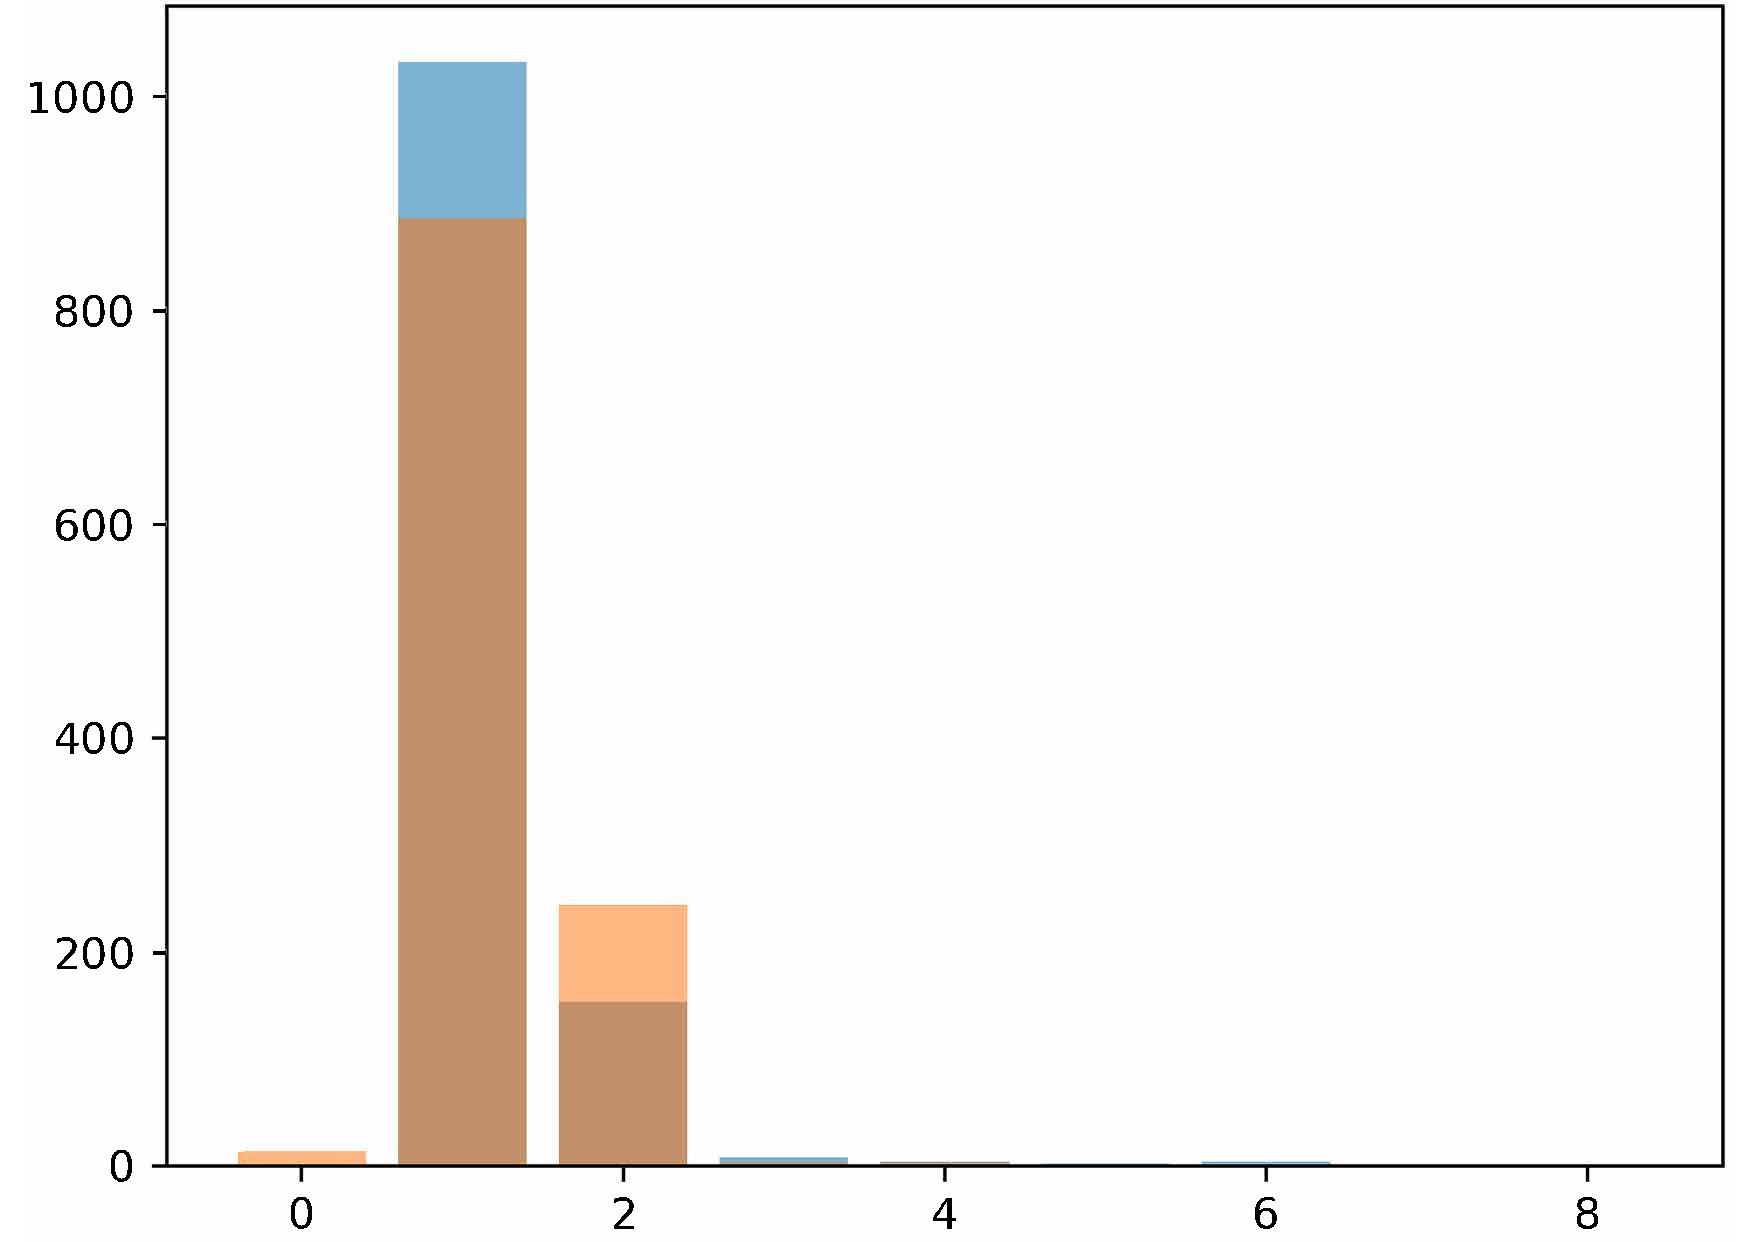
\includegraphics[width=0.23\textwidth,clip=true]{figures/align_hist.pdf}
% }
\subfloat[GagaST]{
    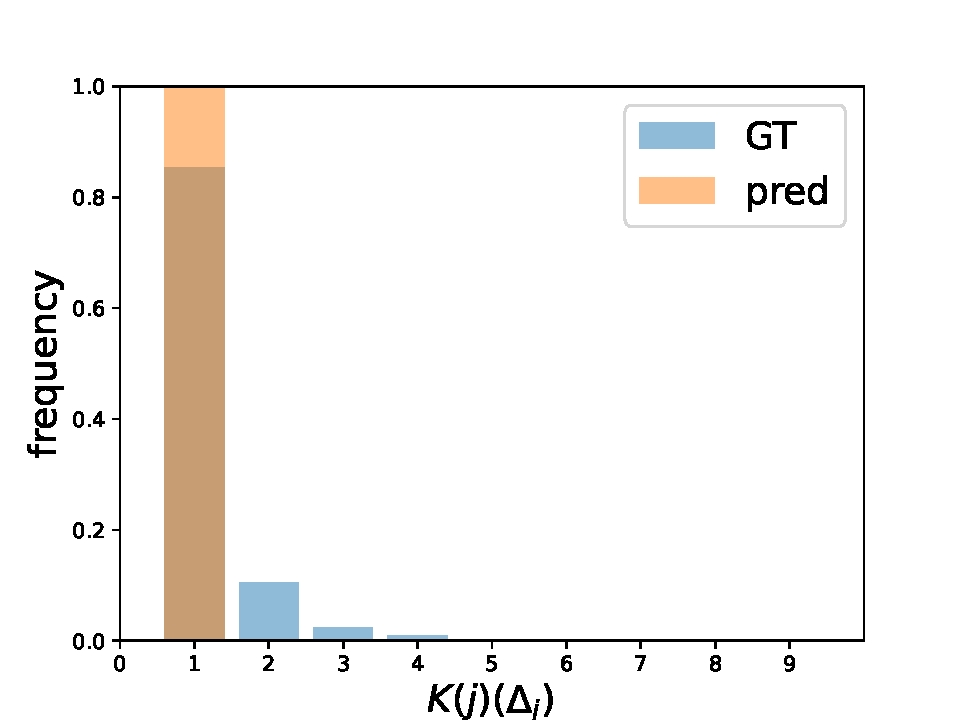
\includegraphics[width=0.49\textwidth,clip=true]{figure/ast/hists/gagast_align_hist.pdf}
}
\subfloat[\modelname-cls]{
    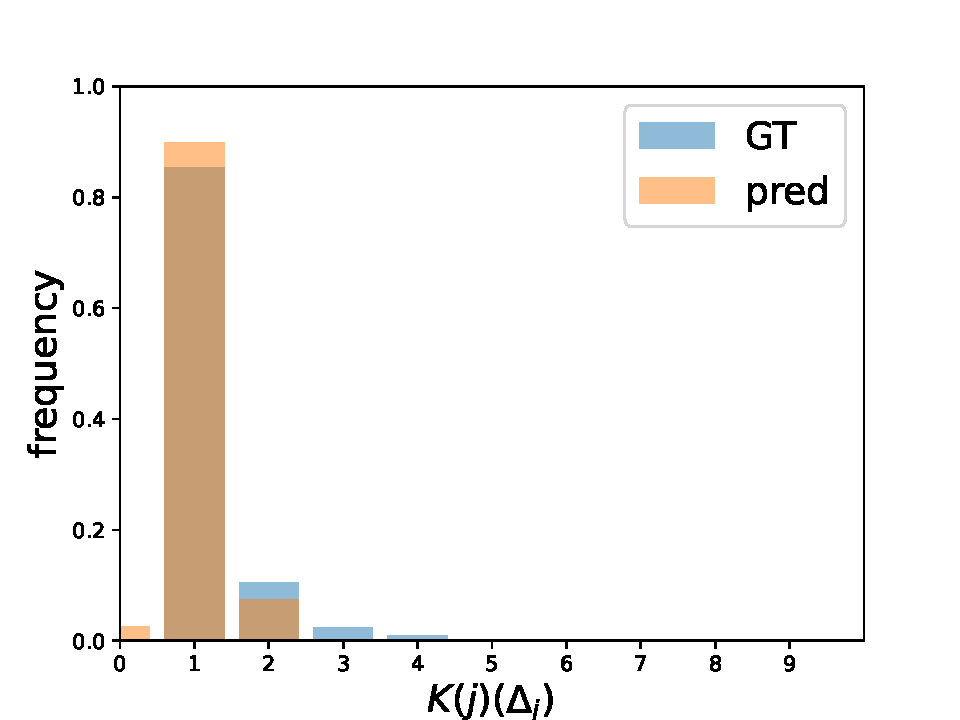
\includegraphics[width=0.49\textwidth,clip=true]{figure/ast/hists/baseline_align_hist.pdf}
}
\caption{En$\rightarrow$Zh方向测试集中的真实歌曲翻译结果对齐情况和模型预测的对齐结果重叠展示的频率分布直方图。}
\label{fig:align_hist1}
\end{figure}
另外,本节还通过使用图\ref{fig:align_hist1}中展示的测试集中的真实歌曲翻译结果对齐情况和模型预测的对齐结果重叠展示的频率分布直方图来观察评估对齐质量。
在表\ref{tab:objective}中,AS列计算了每个模型的直方图与真实直方图之间的对齐分数。
直方图显示,\modelname~生成的对齐的分布类似于真实对齐的分布,而GagaST由于歌词和旋律之间仅提供一对一对齐,因此缺乏多样性。
总之,两个结果都表明,在预测翻译歌词和旋律之间的合理对齐方面,自适应分组方法比长度控制或简单分类器显示出显著优势。
\begin{figure}[ht]
    \centering
\subfloat[GagaST]{
    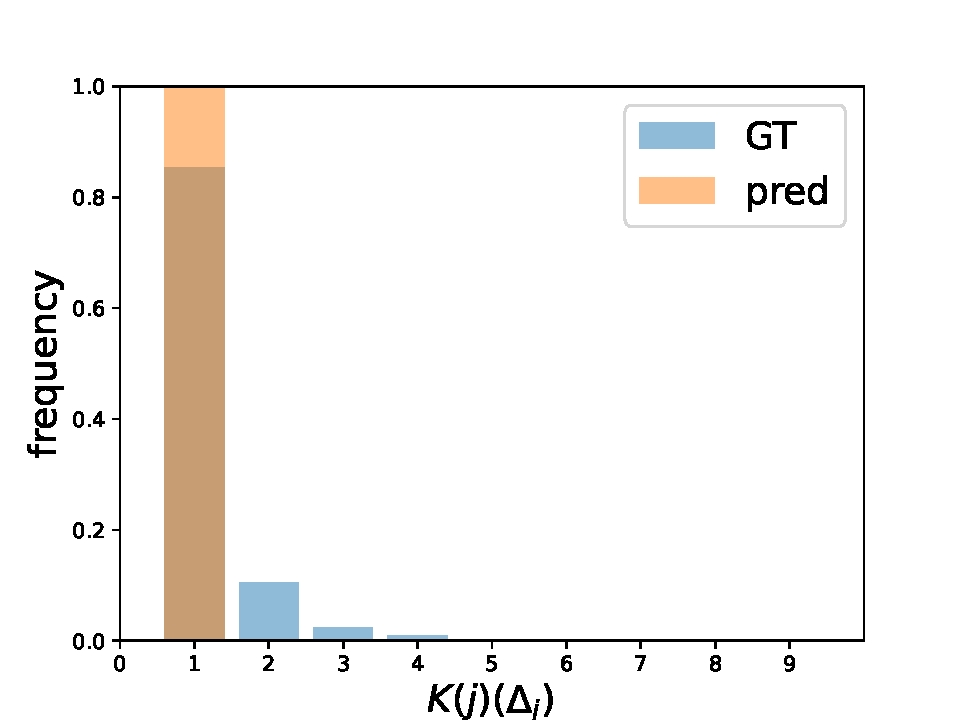
\includegraphics[width=0.49\textwidth,clip=true]{figure/ast/hists/gagast_align_hist.pdf}
}
\subfloat[\modelname]{
    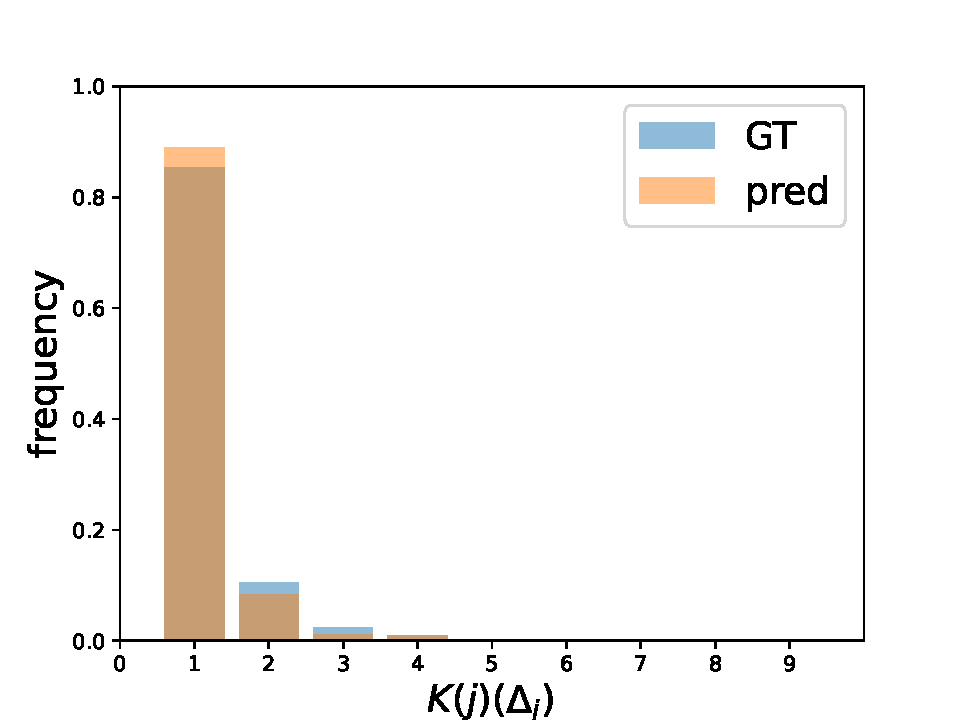
\includegraphics[width=0.49\textwidth,clip=true]{figure/ast/hists/ltag_align_hist.pdf}
}
\caption{En$\rightarrow$Zh方向测试集中的真实歌曲翻译结果对齐情况和模型预测的对齐结果重叠展示的频率分布直方图。}
\label{fig:align_hist2}
\end{figure}
在表\ref{tab:subjective}中,MOS-Q主要反映了歌曲翻译的整体可理解性、自然度、可唱性和美感。
由于歌词文本的翻译和歌词-旋律的对齐的质量都对这一最终结果的评价有影响,因此模型之间的差异似乎不太明显。
但考虑到95\%的置信度区间,这里可以得出结论,\modelname~的表现仍然是最好的。
\subsection{消融实验分析}
首先,本节分析了一些消融实验以研究不同设置下通过回译增强产生的数据的影响。
在表\ref{tab:subjective}中,对\modelname~和\modelname-cls的比较可以得到以下几点发现:
(1)由于回译增强产生的歌曲翻译数据量明显大于真实人工标注的数据量,如果仅使用回译增强产生的翻译数据进行训练,则模型在翻译质量上的表现几乎没有差异。这使得在平行数据非常匮乏和昂贵的情况下,仅使用这样回译产生的数据进行的无监督训练方式就可以很好地满足训练模型翻译能力的需要。
(2)如果只使用数量有限的人工标注监督数据,模型性能会显著下降。这说明模型的容量需要更大的数据量才能进行有效训练,当训练数据不足时,歌词翻译和歌词-旋律对齐的预测性能都会下降,因此,基于back-translation的数据增强手段对于这个任务是很重要的。
(3)\modelname~在这一系列消融实验中的表现始终要比\modelname-cls更好。这说明本章提出的轻量级的对齐解码器结构比一般的分类器有效得多,利用自适应分组算法进行的对齐预测对于歌词-旋律对齐是成功的。
此外,从音符表示池化嵌入层和对齐解码器中移除本章提出的对齐嵌入结构$\mathbf{e}_{align}$的消融实验也验证了这一结构的重要性。从相关实验结果的对比中可以观察到,不使用$\mathbf{e}_{align}$提供的信息,模型翻译的歌曲的BLEU和对齐分数都出现了不可忽略的下降。

\begin{figure}[htbp]
    \centering
\subfloat[源歌谱和参考翻译结果 左图:英$\rightarrow$中。 右图: 中$\rightarrow$英。]{
    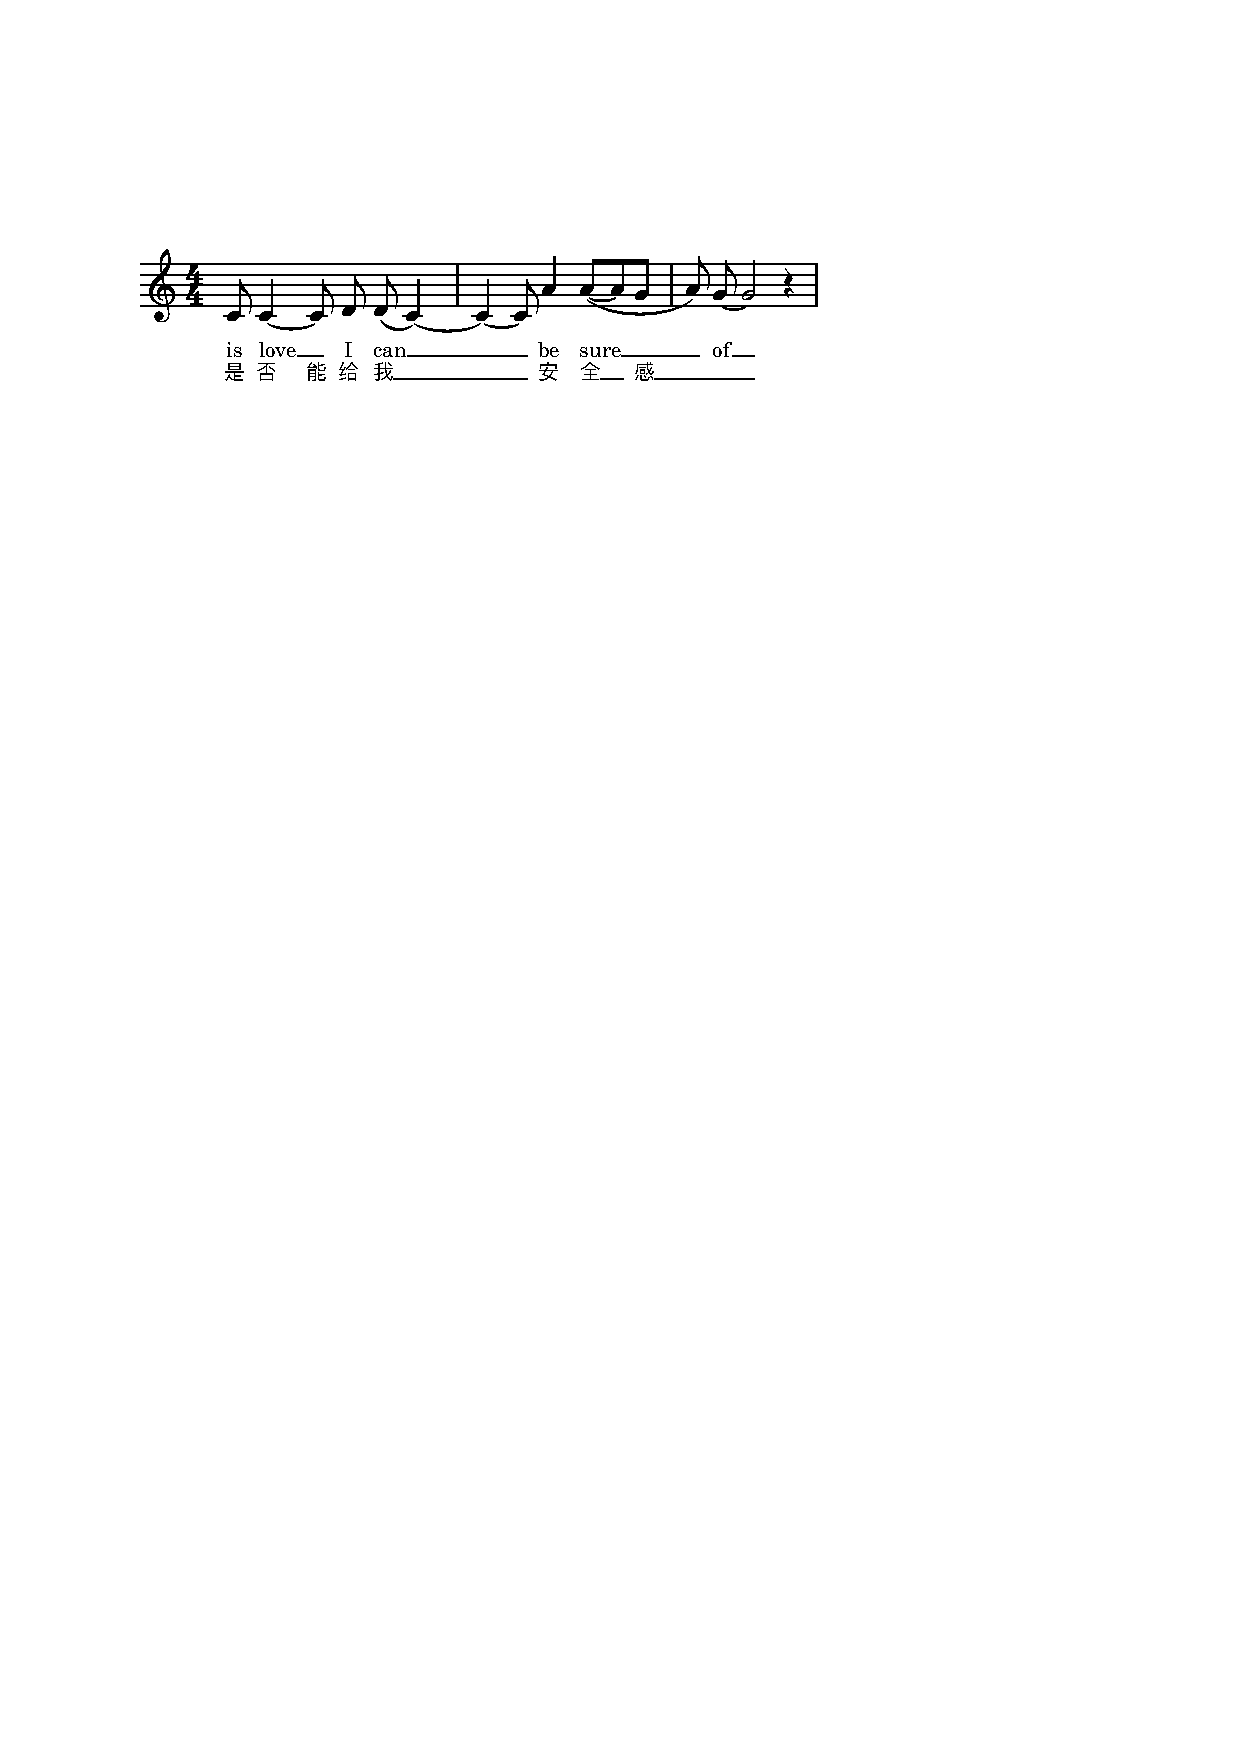
\includegraphics[width=0.55\textwidth,clip=true]{figure/ast/analysis_cases/exp_en_1.pdf}
    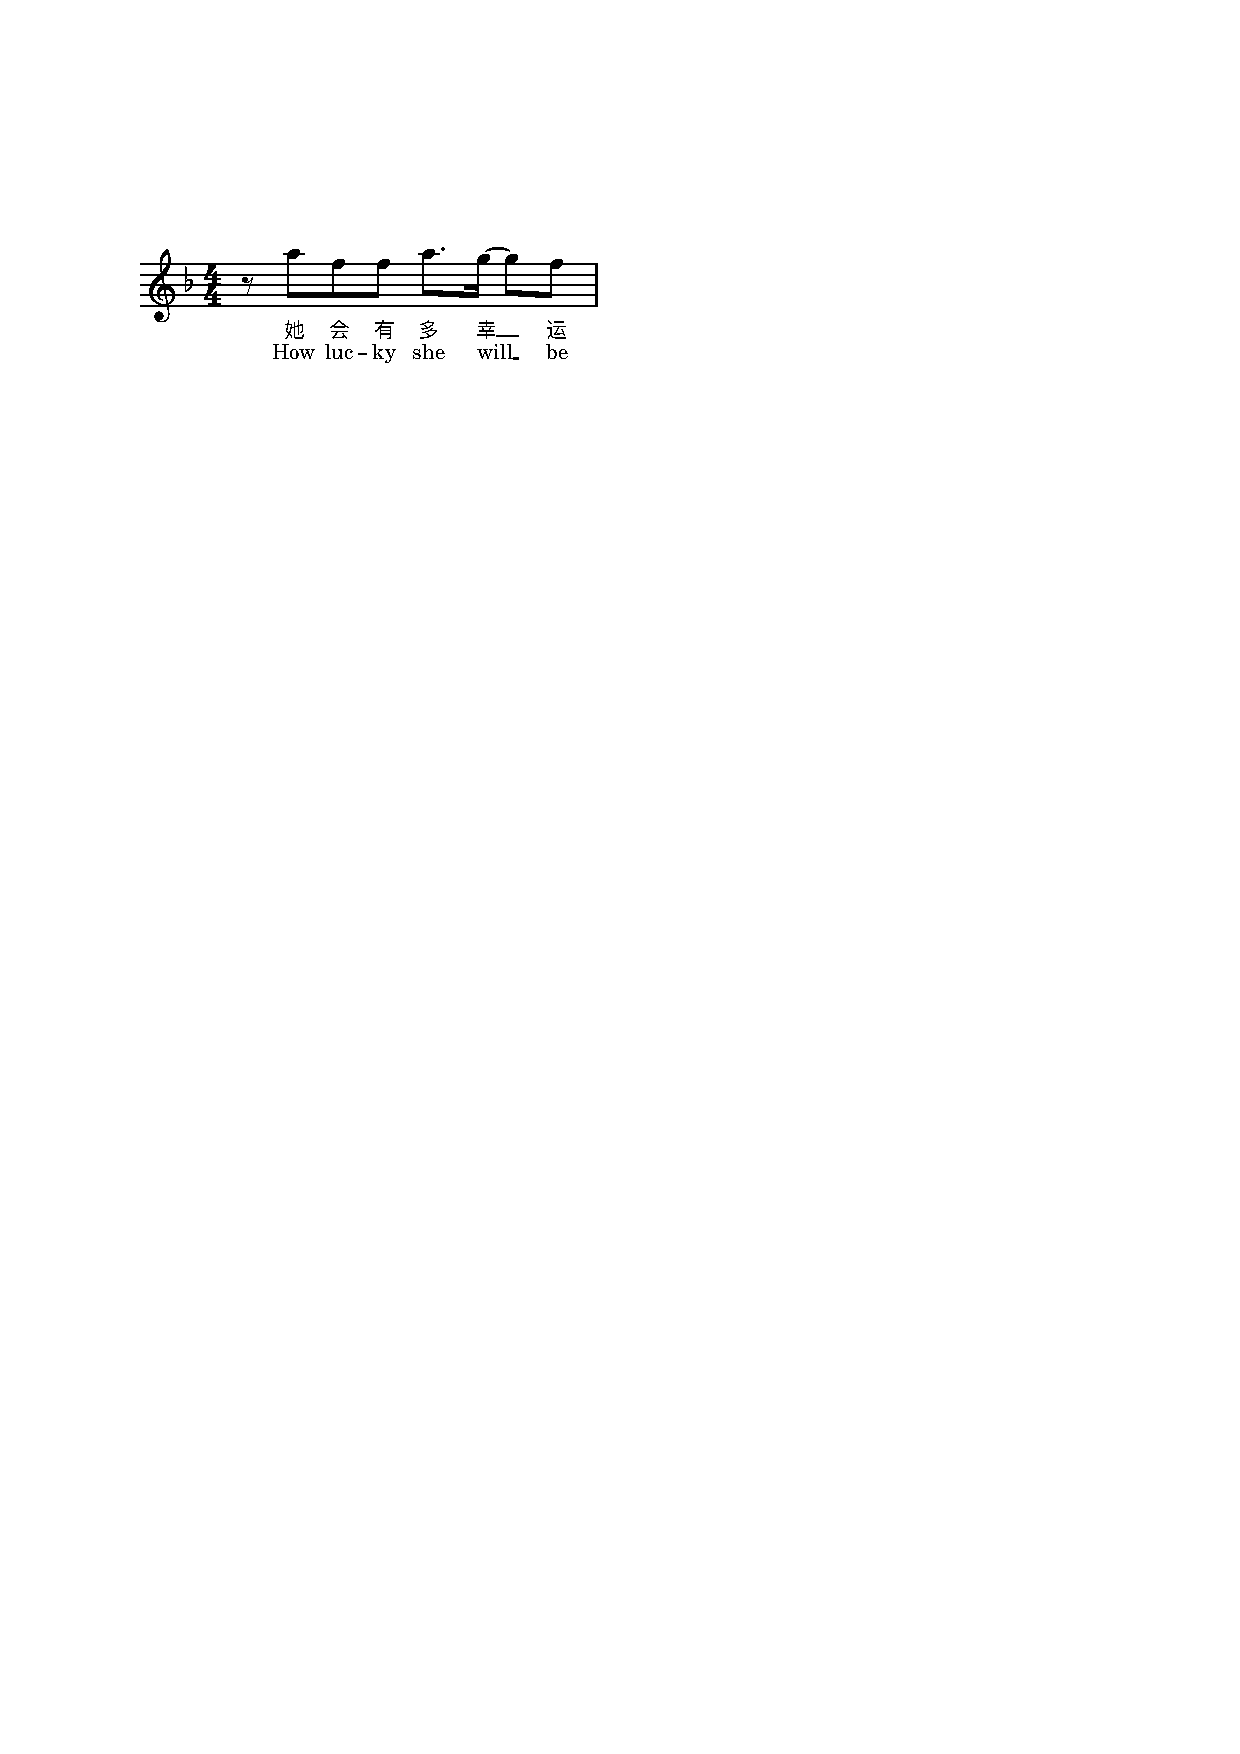
\includegraphics[width=0.43\textwidth,clip=true]{figure/ast/analysis_cases/exp_zh_2.pdf}
}\\
\subfloat[GagaST]{
    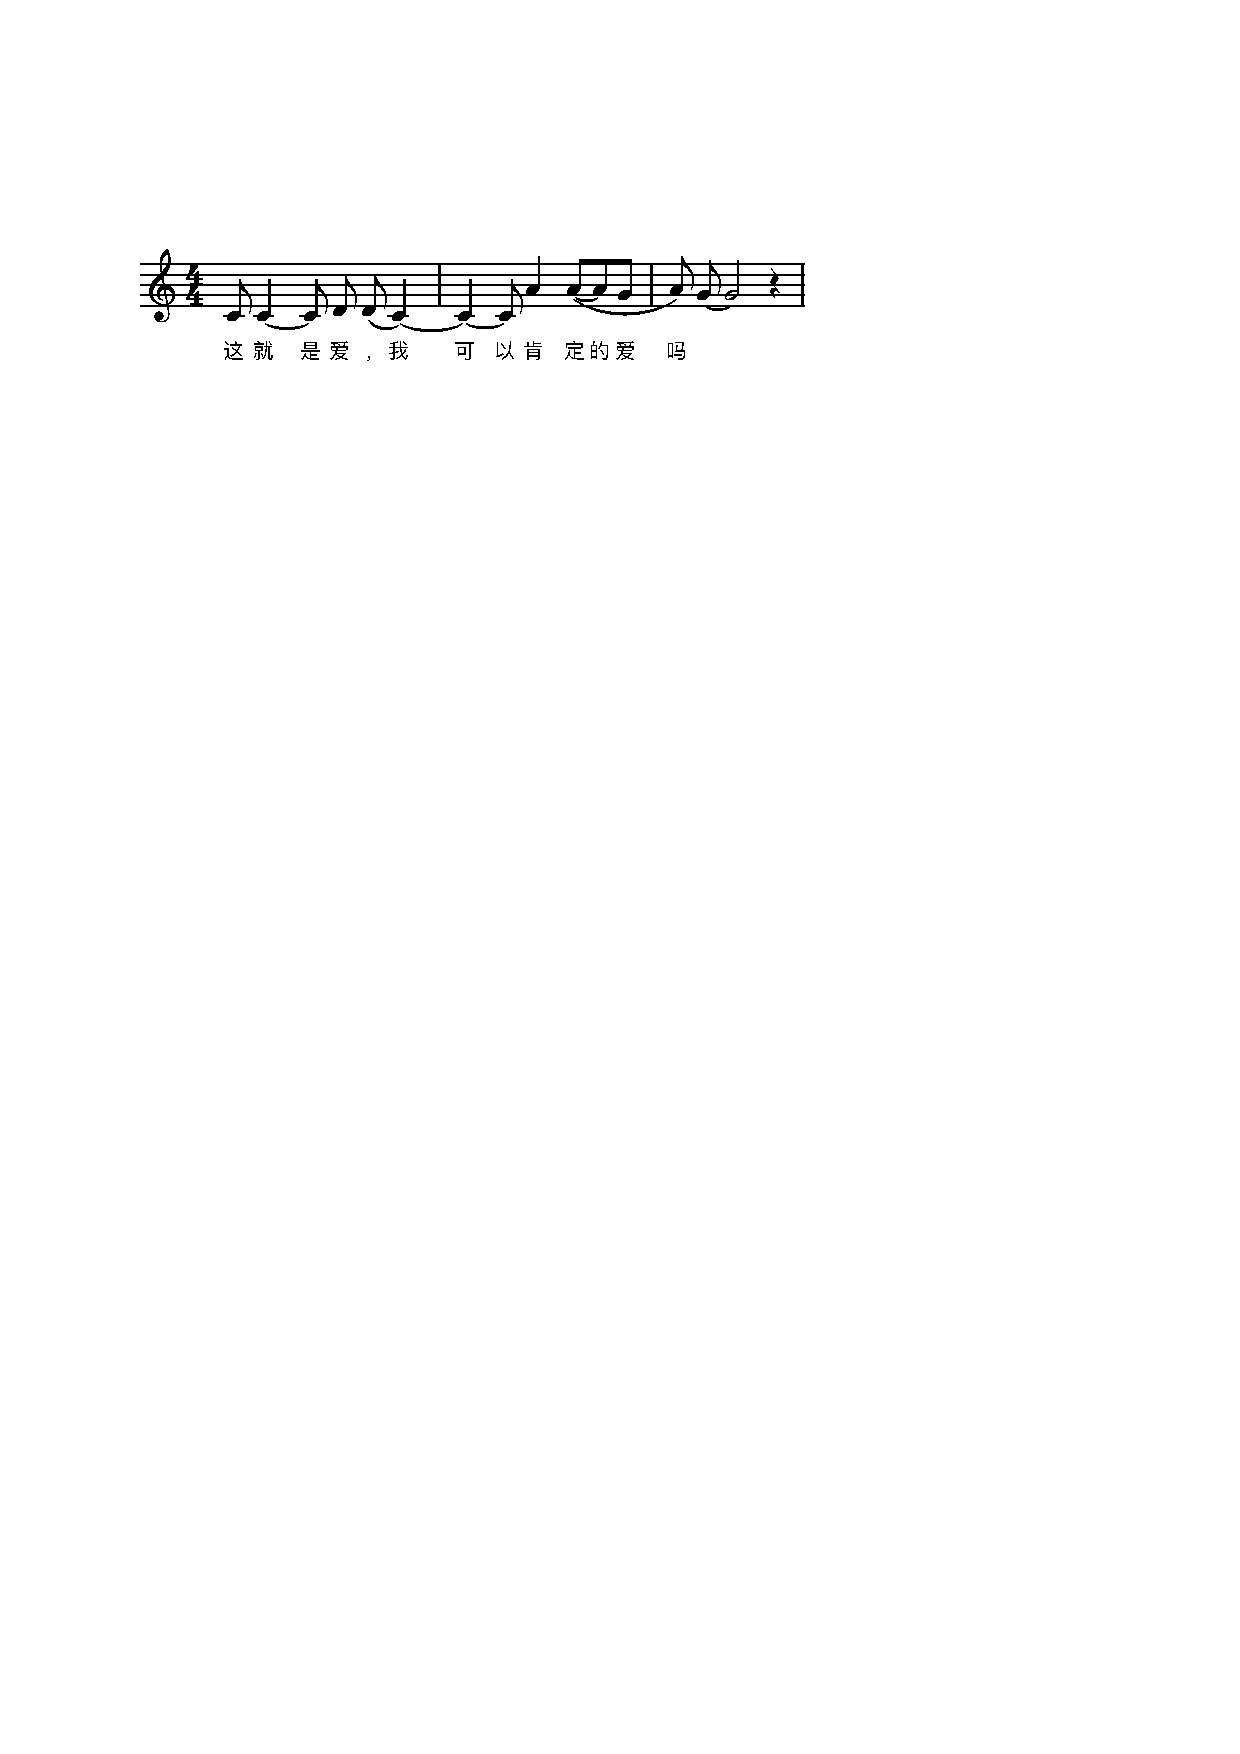
\includegraphics[width=0.55\textwidth,clip=true]{figure/ast/analysis_cases/exp_gagast_zh_1.pdf}
    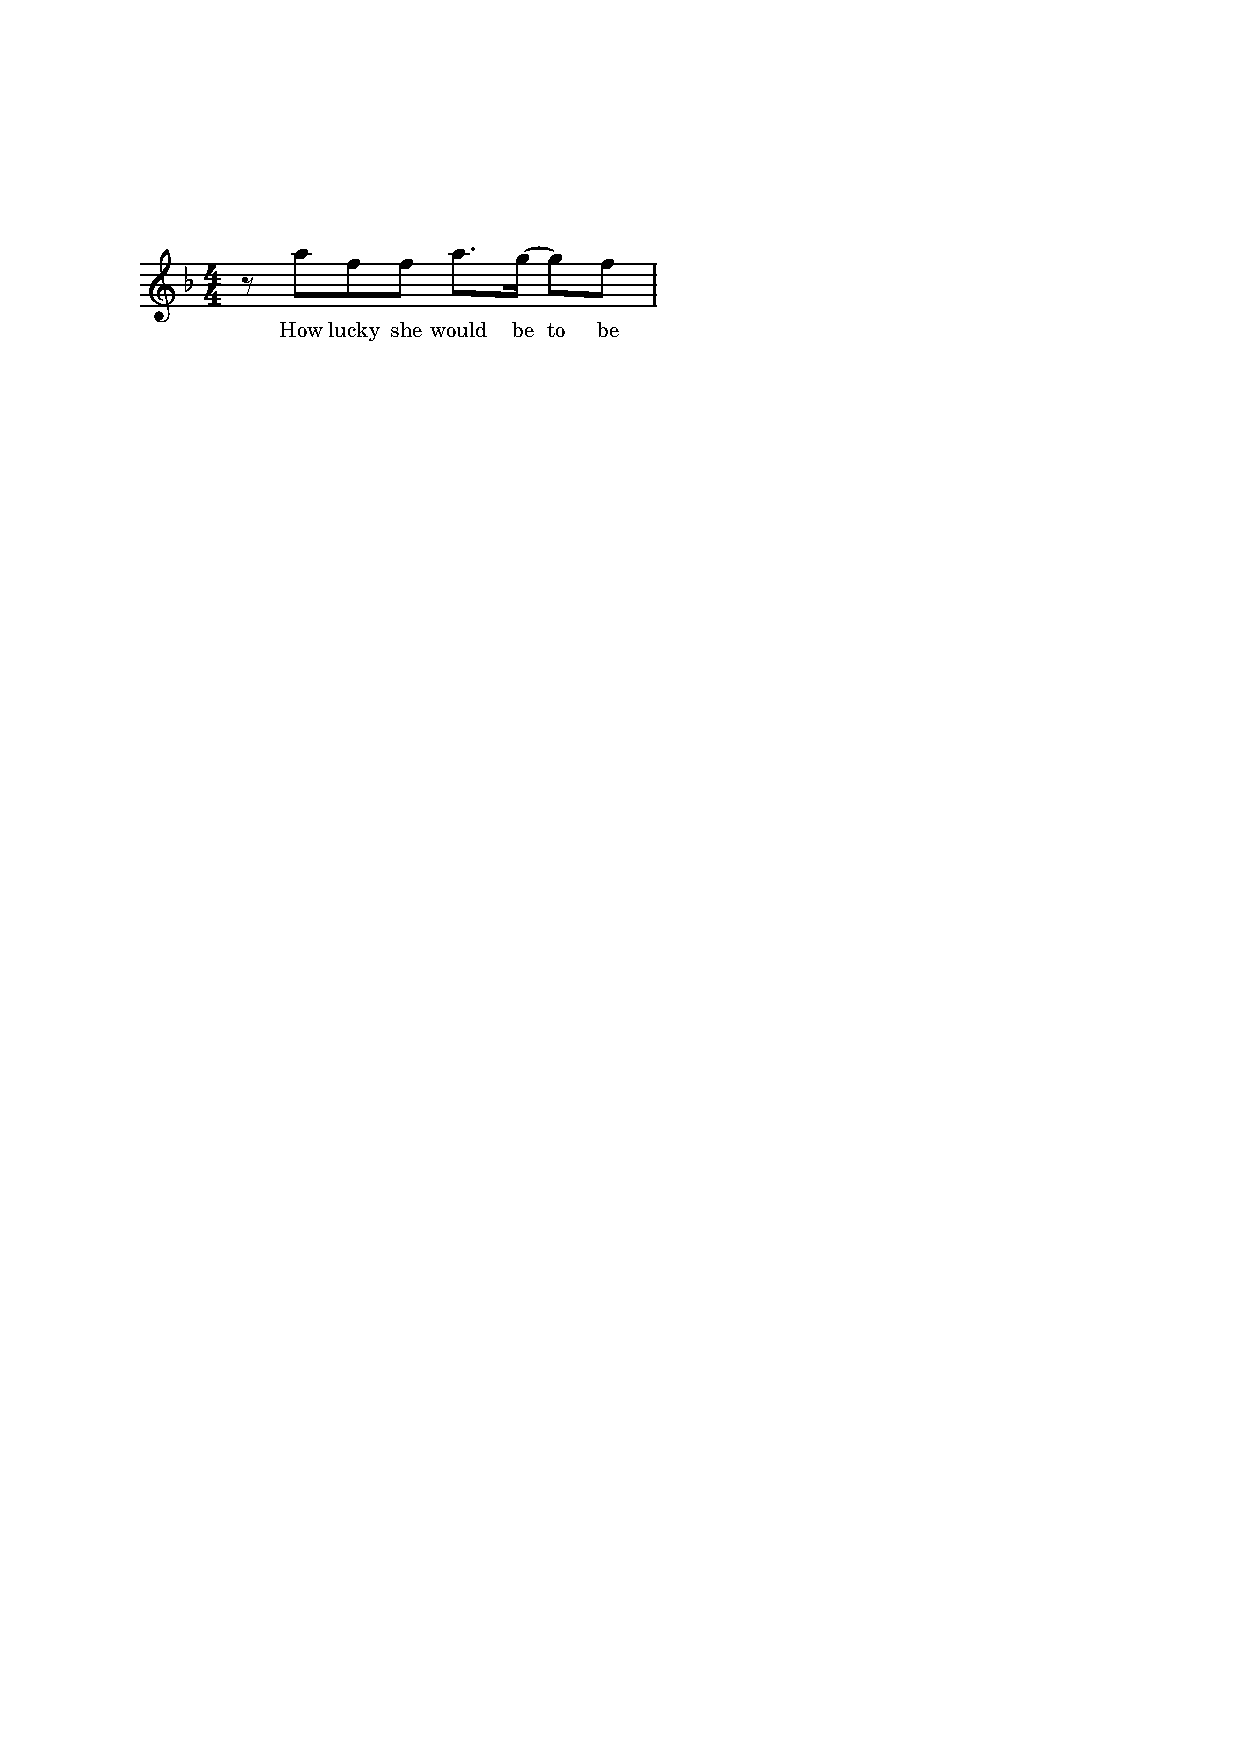
\includegraphics[width=0.44\textwidth,clip=true]{figure/ast/analysis_cases/exp_gagast_en_2.pdf}
}\\
\subfloat[\modelname-cls]{
    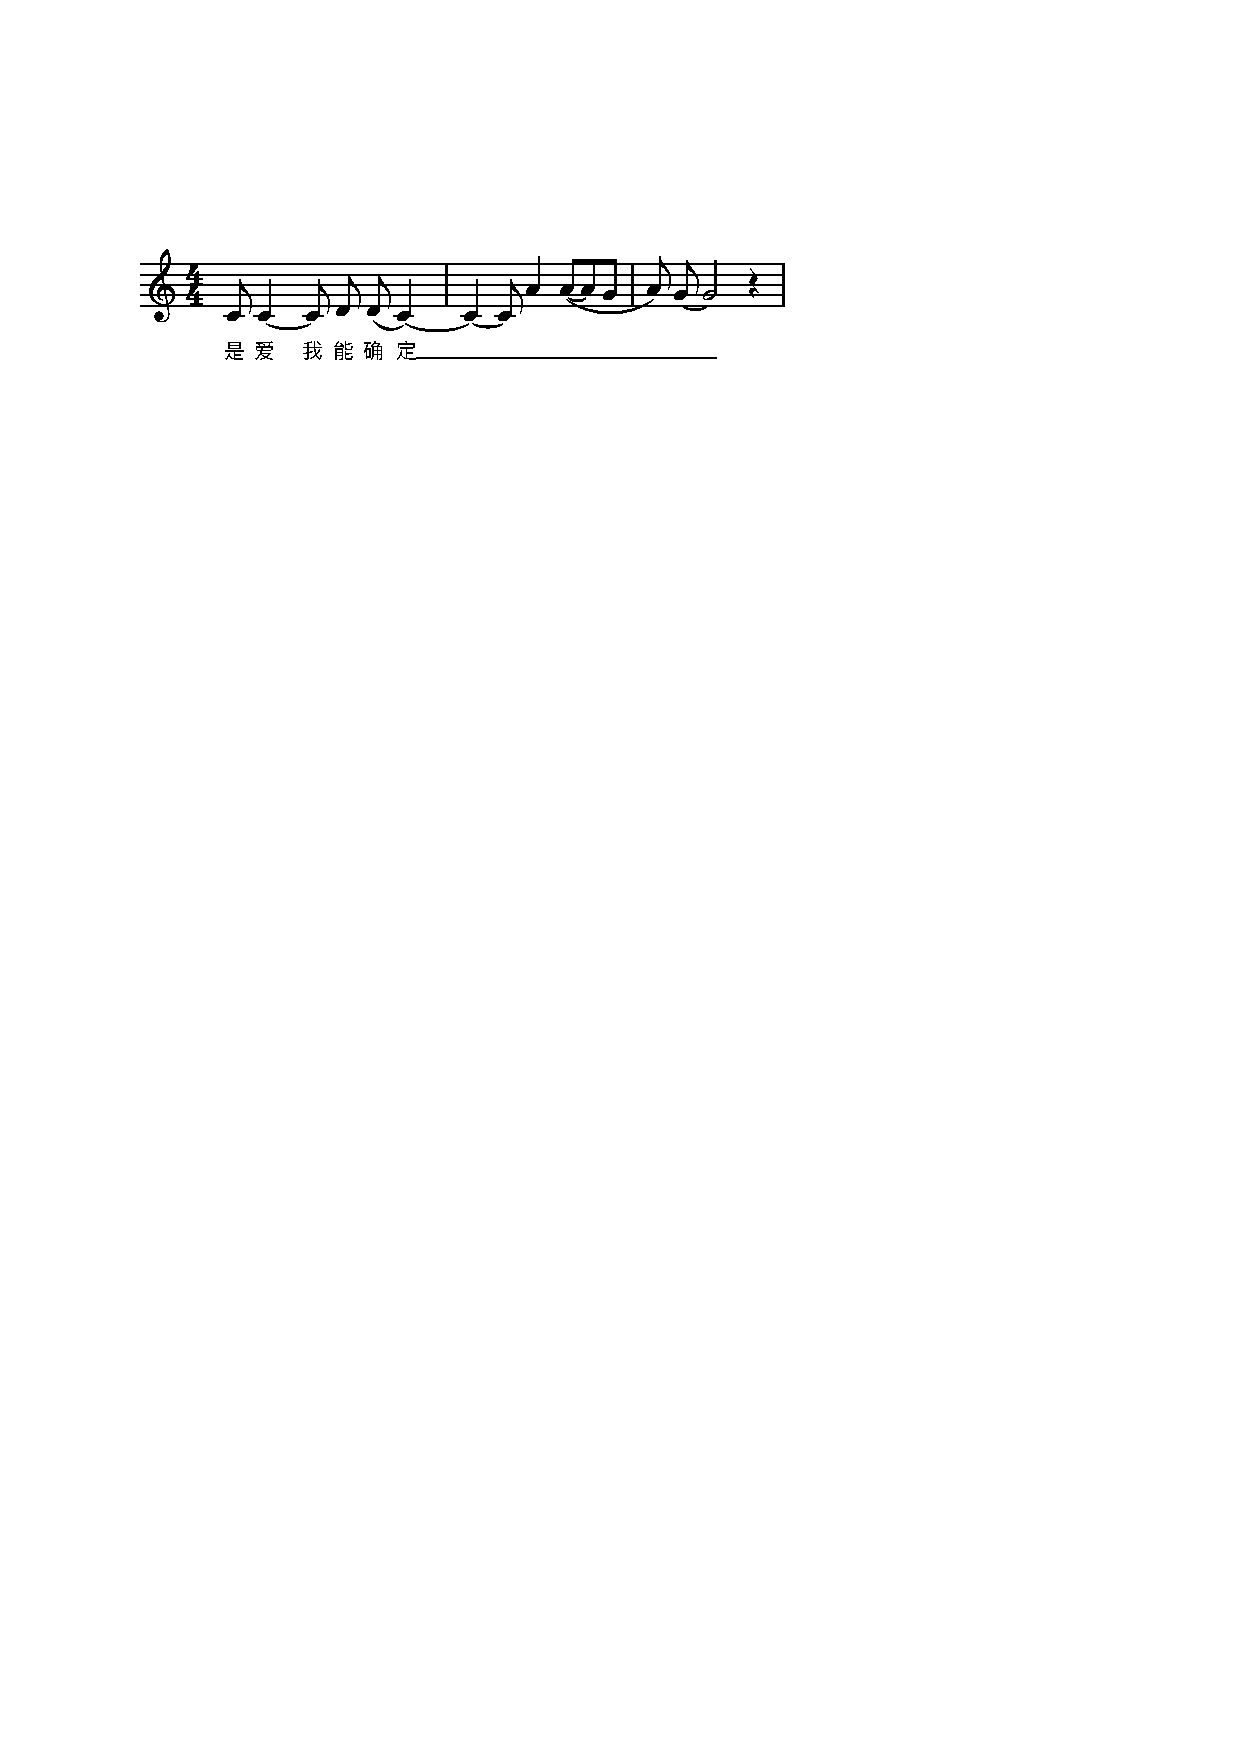
\includegraphics[width=0.55\textwidth,clip=true]{figure/ast/analysis_cases/exp_baseline_zh_1.pdf}
    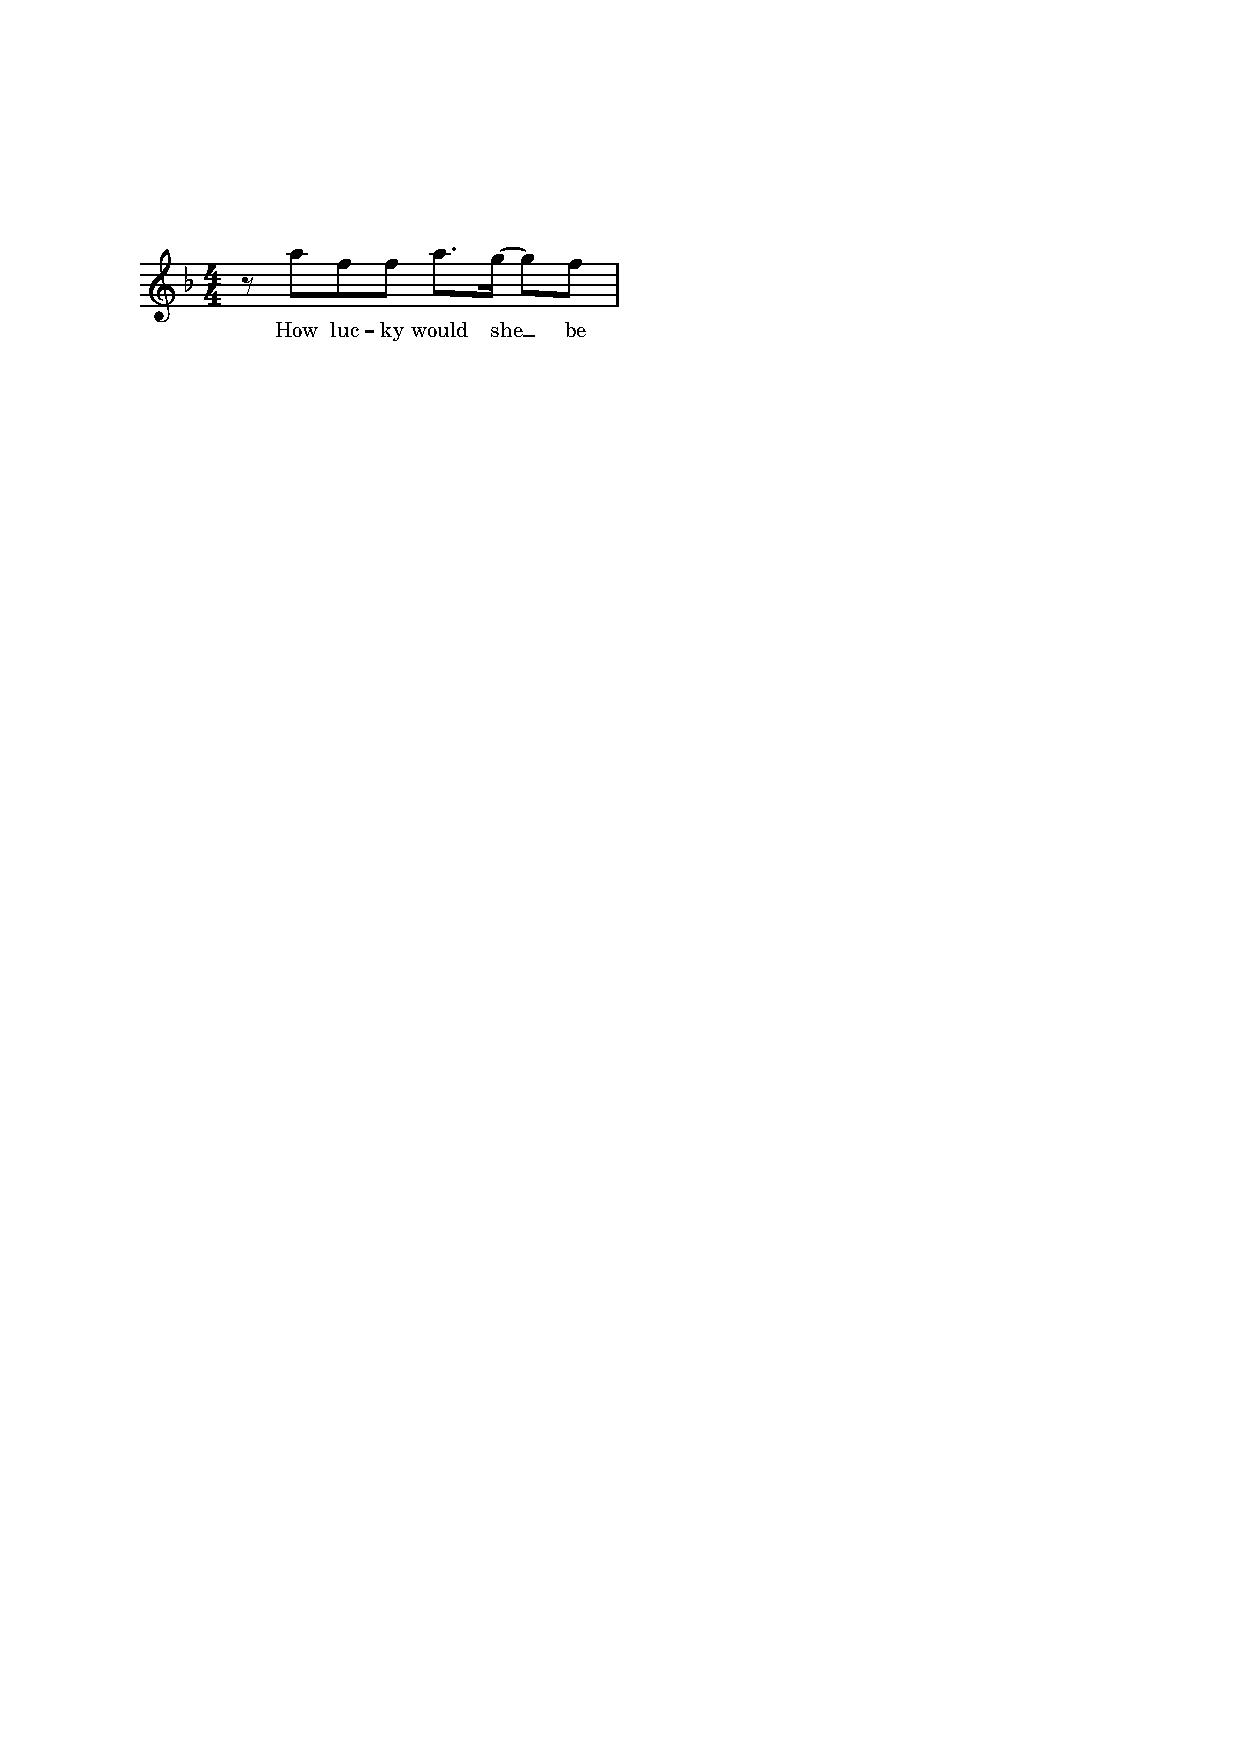
\includegraphics[width=0.44\textwidth,clip=true]{figure/ast/analysis_cases/exp_baseline_en_2.pdf}
}\\
\subfloat[\modelname]{
    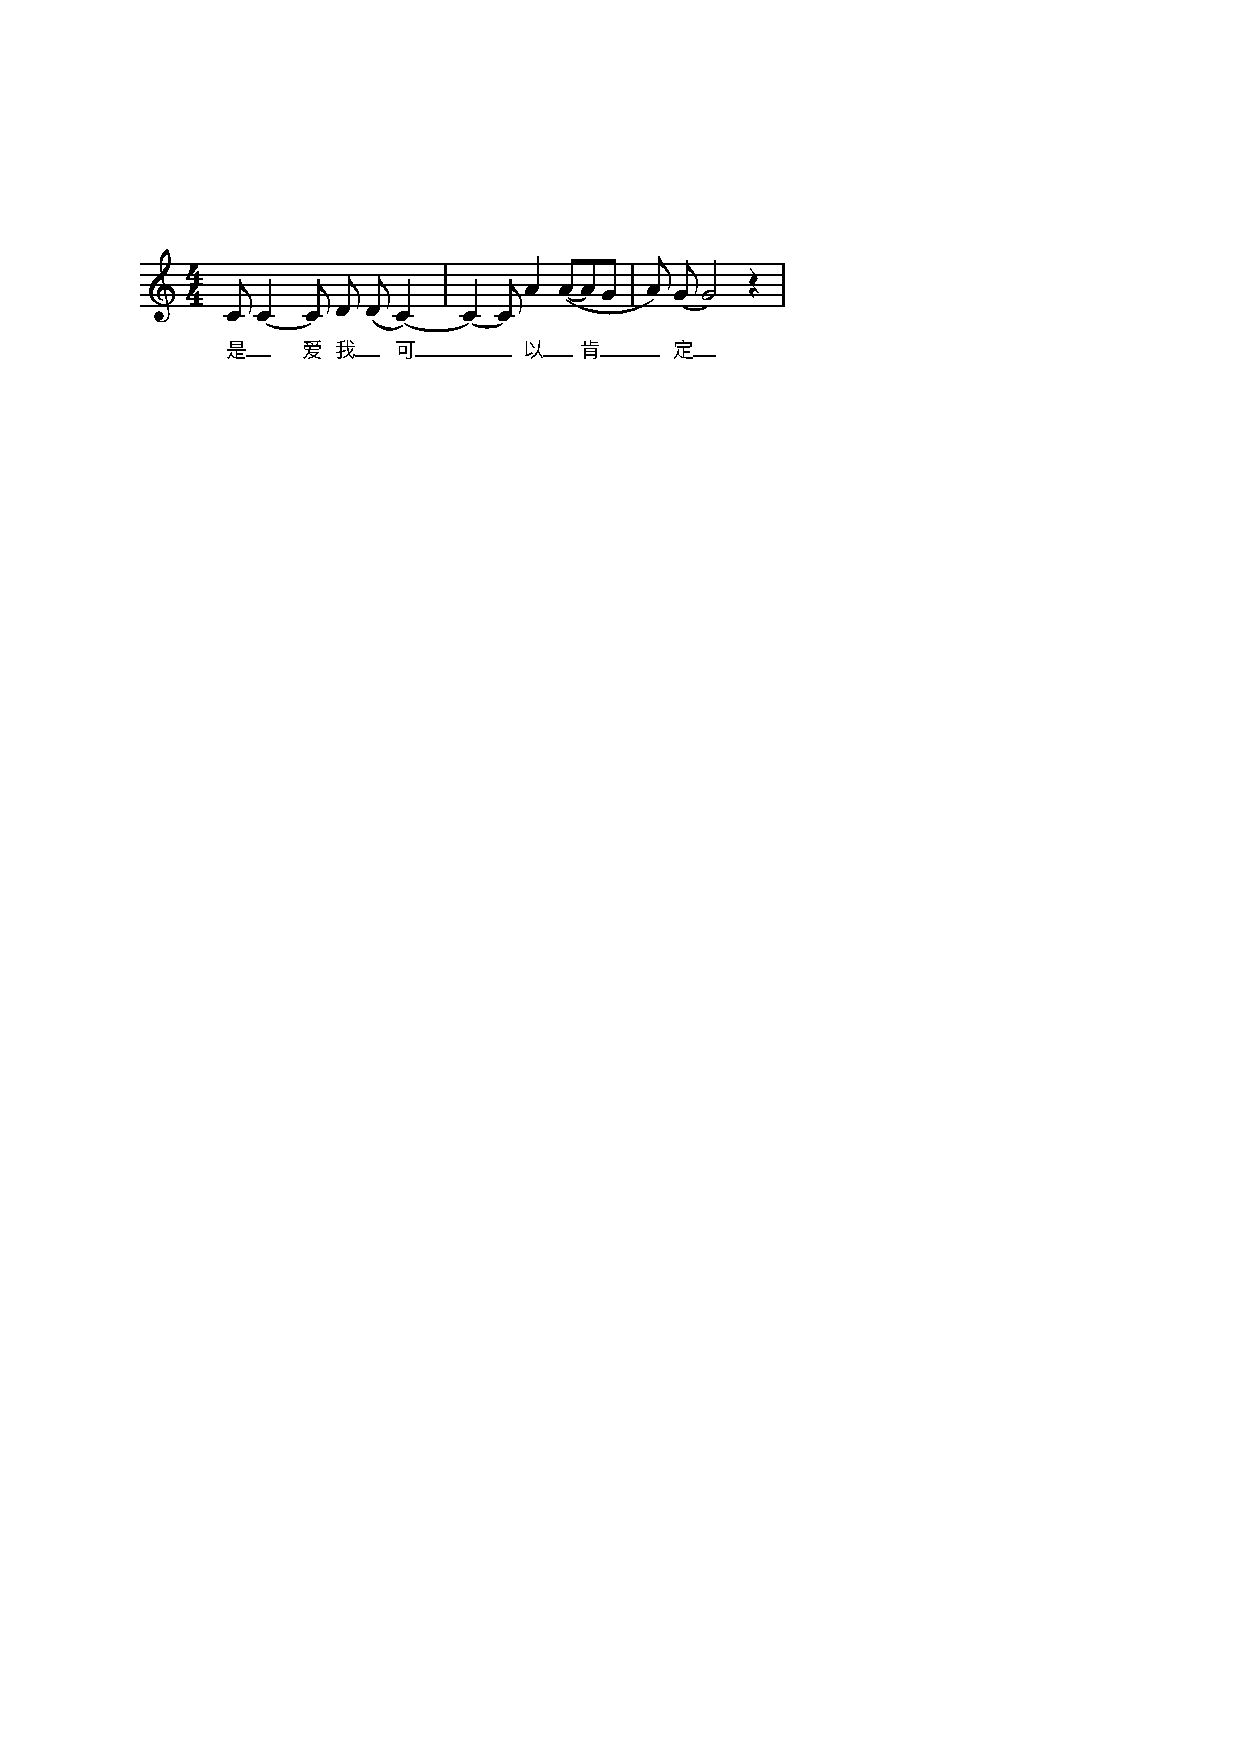
\includegraphics[width=0.55\textwidth,clip=true]{figure/ast/analysis_cases/exp_LTAG_zh_1.pdf}
    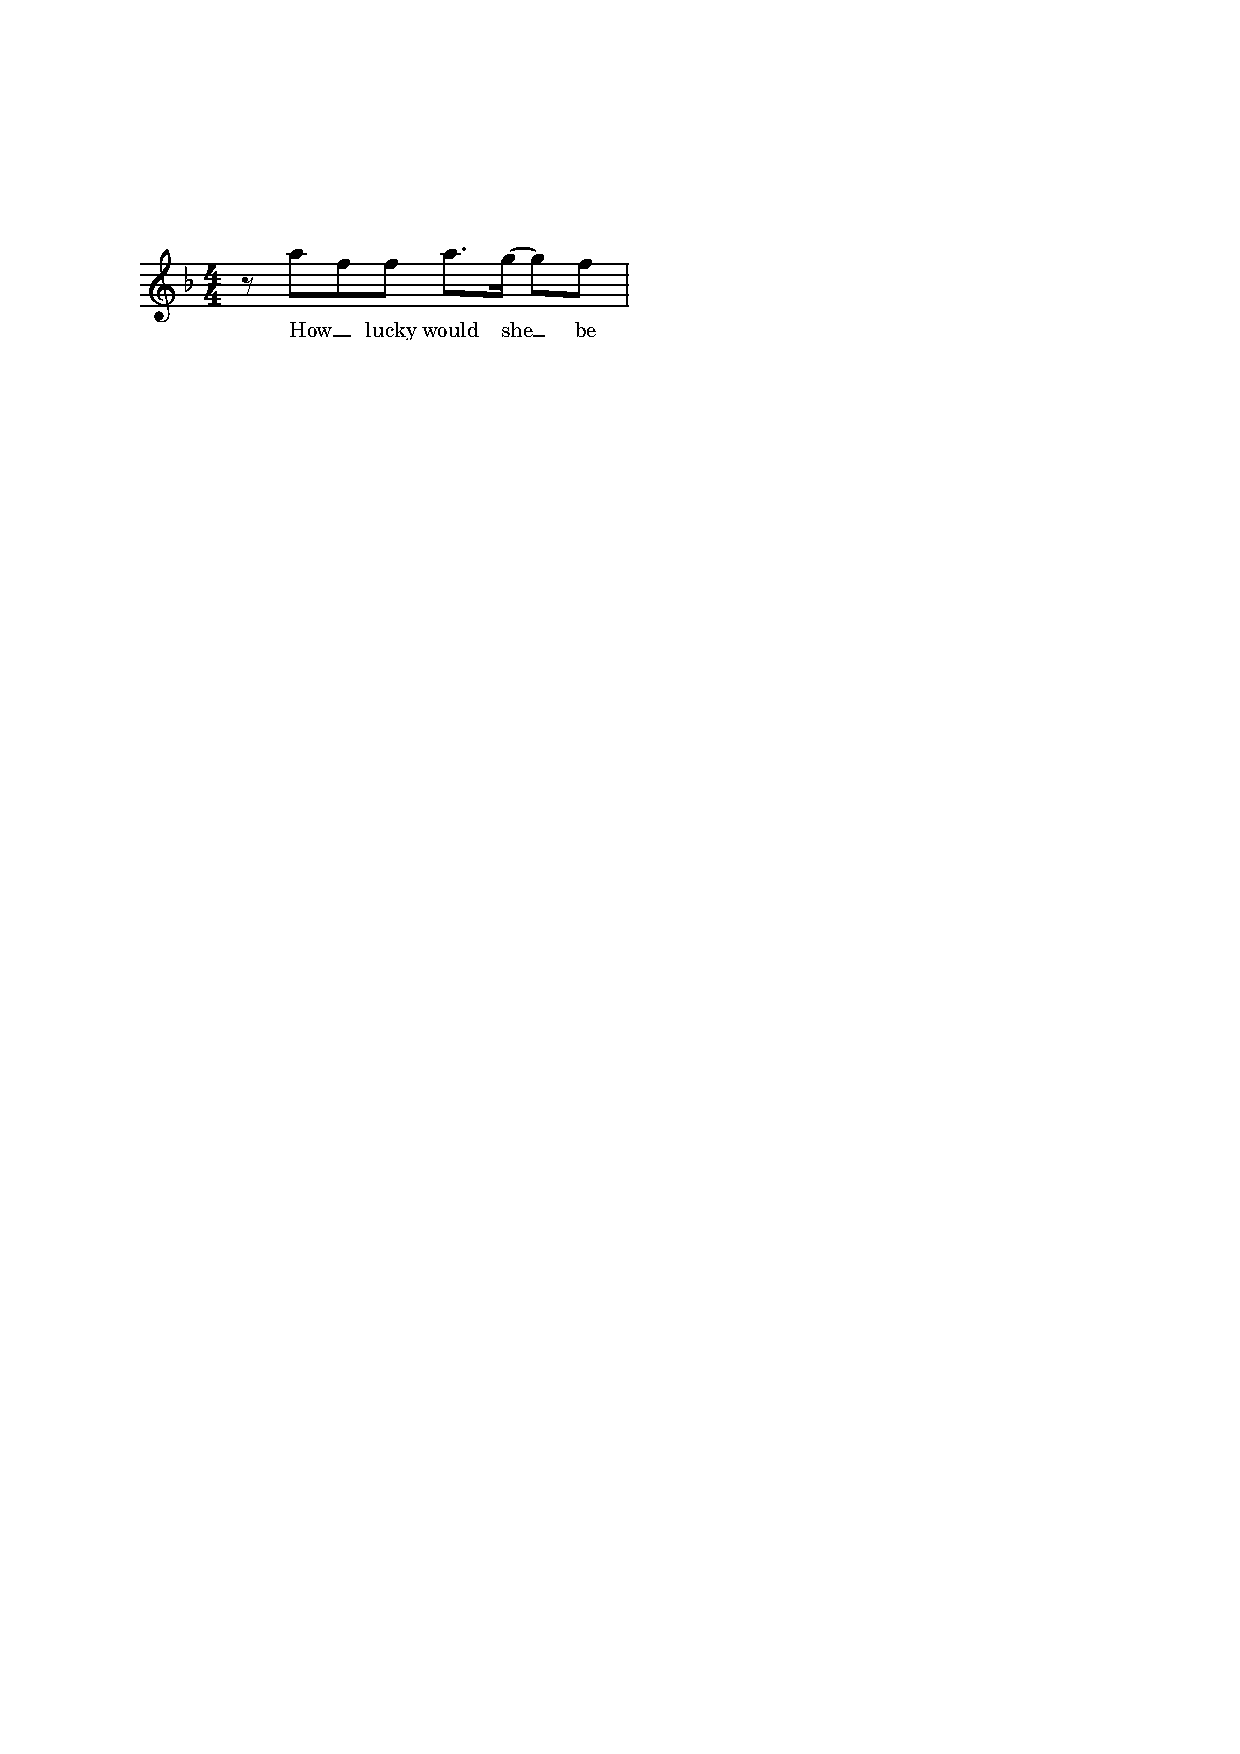
\includegraphics[width=0.44\textwidth,clip=true]{figure/ast/analysis_cases/exp_LTAG_en_2.pdf}
}\\
\caption{源歌词、参考翻译结果和本章中进行比较的三个歌曲翻译模型的翻译结果的歌谱示例。两个例子分别为《\textit{Will You Love Me Tomorrow}》一曲中的``Is love I can be sure of''和《\textit{小幸运}》一曲中的``她会有多幸运''。}
\label{fig:score_analysis}
\end{figure}
图\ref{fig:score_analysis}中展示了一些具体的翻译案例。根据翻译案例的示例,当源歌词中的词语和音符出现一对多对齐的情况时(源曲中的``love''、``can''、``sure''和``运''等),GagaST通常会因为需要满足解码长度限制而给出不太合适的歌词翻译,甚至会解码出不发声的富豪,如逗号或句号等,这既损害了翻译质量,又影响了翻译歌词的可唱性。
这种现象的原因就在于源曲在表达此句的意思时,部分歌词出现了一对多对齐的情况,此时音符的数量相比字词已经过多了,解码时的限制就变成了用更多字数表达相同的意思,对齐情况受限的模型只能添加更多无语义的字词语或者不合适的词语来满足限制。
相比之下,Transformer子结构+简单分类器的\modelname-cls~已经可以实现相对灵活的对齐了。
然而,实验评估结果表明,本章提出的轻量的对齐解码器网络结构能够在目标端词语和音符之间预测出更合理的对齐。
\section{本章小结}
本章主要针对自动歌曲翻译任务提出了一个可以同时考虑歌词和歌词-旋律对齐情况来进行翻译的自回归模型。本章提出的歌词和歌词-旋律对齐共同翻译模型LTAG是在自回归的基于Transformer的编码器-解码器翻译框架下的改进。本章细致阐述了模型的设计动机,介绍了本章提出的数据收集方法、实验中使用的数据集情况、本章提出的音符表示池化嵌入层和对齐解码器的具体结构。最后,通过一系列实验和翻译结果的歌谱分析,本章说明了\modelname~相比两个很强的基线模型取得了更好的文本语义翻译表现和更为合理、更有表现力的歌词-旋律对齐,从而获得了整体上更好的歌曲翻译表现,模型有能力为翻唱提供了优质的歌词和歌谱参照。
